\documentclass[a4paper,12pt]{report}
\usepackage{mathptmx}
\usepackage[margin=1in]{geometry}
\linespread{1.25}
\usepackage[utf8]{inputenc}
\usepackage{amsmath}
\usepackage[maxbibnames=9, backend=biber]{biblatex}
\usepackage{graphicx}
\usepackage[Symbol]{upgreek}
\usepackage{listings}
\usepackage{pythonhighlight}
\usepackage{wasysym}
\usepackage{url}
\usepackage{color}
\usepackage[hidelinks]{hyperref}
\usepackage{indentfirst}
\DeclareFieldFormat*{title}{\mkbibemph{#1}}
\DeclareFieldFormat{urldate}{(accesat în #1)}
\DeclareFieldFormat{pages}{pag. #1}
\DeclareLanguageMapping{english}{UKenglish}
\def\UrlBreaks{\do\/\do-}
\setcounter{biburllcpenalty}{7000}
\setcounter{biburlucpenalty}{8000}
\lstset{basicstyle=\ttfamily\footnotesize,breaklines=true}

\addbibresource{biblio.bib}
\renewcommand{\chaptername}{Capitolul}
\renewcommand{\figurename}{Figura}
\renewcommand{\tablename}{Tabelul}

\definecolor{dkgreen}{rgb}{0,0.6,0}
\definecolor{gray}{rgb}{0.5,0.5,0.5}
\definecolor{mauve}{rgb}{0.58,0,0.82}
\definecolor{gray}{rgb}{0.4,0.4,0.4}
\definecolor{darkblue}{rgb}{0.0,0.0,0.6}
\definecolor{lightblue}{rgb}{0.0,0.0,0.9}
\definecolor{cyan}{rgb}{0.0,0.6,0.6}
\definecolor{darkred}{rgb}{0.6,0.0,0.0}
\lstdefinelanguage{XML}
{
  morestring=[s][\color{dkgreen}]{"}{"},
  morestring=[s][\color{black}]{>}{<},
  morecomment=[s]{<?}{?>},
  morecomment=[s][\color{dkgreen}]{<!--}{-->},
  stringstyle=\color{black},
  identifierstyle=\color{lightblue},
  keywordstyle=\color{mauve},
  morekeywords={xmlns, xsi, noNamespaceSchemaLocation, type, id, x, y, source, target, version, 
  tool, transRef, roleRef, objective, eventually, app, android}
}

\begin{document}

\begin{titlepage}
    \begin{center}
        
        \vspace{0.5cm}
        \textbf{\Large UNIVERSITATEA BABEŞ-BOLYAI CLUJ-NAPOCA} \\
        \vspace{0.5cm}
        \textbf{\Large FACULTATEA DE MATEMATICǍ ŞI INFORMATICǍ} \\
        \vspace{0.5cm}
        \textbf{\Large SPECIALIZAREA INFORMATICĂ ROMÂNĂ}    
        
        \vspace{4cm}
        \textbf{\LARGE LUCRARE DE LICENȚĂ}
        
        \textbf{\Huge RECUNOAȘTEREA AUTOMATĂ A PARTITURILOR MUZICALE}
       
    \end{center}

    \vspace{5.5cm}
    \begin{flushleft}

        \textbf{\LARGE Conducător științific}

        \textbf{\LARGE Conf. univ. dr. Grigoreta Sofia Cojocar}
        
    \end{flushleft}
    
    \vspace{1cm}
    \begin{flushright}

        \textbf{\LARGE Absolvent}

        \textbf{\LARGE Răzvan Cosmin Linca}

    \end{flushright}

    \vspace{0.8cm}
    \begin{center}
        \textbf{\Large Cluj-Napoca}

        \textbf{\Large 2020}
    \end{center}

 \end{titlepage}
 \chapter*{Abstract}

The past few years have brought a significant increase in 
interest for acoustic music, 
closely related to the parallel evolution of technology globally, 
with focus on social networks and video streaming.

It was found that the evolution determined a distance between
performers and the musical sheet, as the process of learning through 
online tutorials has become much easier. 
Also, the classical sheet is a musical element with high difficulty, 
being necessary to know some notions of music theory for a full understanding.
Therefore, it proved necessary to use a simple and suggestive notation, 
specific to acoustic music, namely musical tabulature.

Given the existence of these limitations and the desire of guitarists, 
one solution would be the existence of a platform through which acoustic 
parts can be transcribed automatically, directly into a tabular representation,
using guitar chords. 

The first step of the automatic chord recognition system (ACR) is to 
apply a sound processing method, in order to extract important musical 
features, by using a suitable representation in the field, namely chromagram.
This first step is a vital one in the analysis of a musical sample, 
as obtaining a correct representation is closely related to 
the continuous development of the system. 

The second part defines the algorithms that 
underlie the learning processes and differentiate the 
features of some chords from a musical sample, specifically, 
machine learning algorithms. The goal is to gradually arrive at a complex 
and up-to-date machine learning algorithm, able to automatically and independently 
analyze the audio signal and to classify with high 
precision each sequence within an acoustic sample.

In order to highlight the good functioning of the ACR, 
the system will be connected with a mobile application, 
intended for acoustic music enthusiasts. The application will be able to display, 
in real time, the results of the automatic recognition of acoustic musical chords, 
for any desired musical sheet.

\newpage

\newpage
\renewcommand{\contentsname}{Cuprins}
\tableofcontents
\chapter{Introducere}
Muzica acustică contemporană se află într-o perioadă de creștere din punct de vedere 
tehnologic, odată cu evoluția paralelă a rețelelor de socializare(platforme 
video și de streaming, platforme de socializare ș.a.m.d), care au conectat
artiști profesioniști și amatori ai domeniului.

Această evoloție a determinat o îndepărtare a interpretului de partitură, acesta fiind ori un artist profesionist care
învață un cântec prin simpla ascultare sau vizualizare a unei înregistrări, sau un amator
pasionat care învață prin urmărirea repetată a unor tutoriale aflate pe platformele
online. De altfel, este cunoscut faptul că mulți compozitori și chitariști renumiți nu puteau
să citească sau să scrie partituri muzicale, bazându-se pe talentul muzical 
în a memora fragmente sau a improviza pe loc diverse ritmuri.
Printre ei se numără Jimi Hendrix, Eric Clapton, Elvis Presley sau
interpreții trupei The Beatles \cite{WEBSITE:the-music-studio}.

Chitariștii susțin că notația clasică prin partitură muzicală este foarte bine orientată
către instrumente cu clape, cum ar fi pianul, fiind în general neutilizată pentru chitară. 
Pe de altă parte, notația prin tabulatură este optimizată pentru instrumentele cu corzi și
freturi, fiind de folos mai mare pentru aceștia. Cu toate acestea, o cantitate uriașă de 
piese au fost scrise doar în notația clasică prin partitură, iar transcrierea unei piese
de la partitură la o tabulatură corectă este un proces complex care necesită cunoștințe 
de specialitate. Prin urmare, materialul devine inaccesibil pentru chitariștii aspiranți care
nu sunt atât de specializați.

Având în vedere existența acestor limitări și dorința chitariștilor, o soluție 
ar fi existența unei platforme prin intermediul căreia se pot transcrie piese 
acustice, în mod automat, direct într-o reprezentare prin tabulatură, specifică
instrumentelor cu corzi.

Astfel, subiectul propus urmărește implementarea unei platforme pentru telefoane
mobile, care să permită transpunerea automată a unor interpretări la chitară acustică, într-o
reprezentare simplă și sugestivă pentru orice posibil interpret. Algoritmul 
de automatizare va avea la bază un algoritm de învățare automată, din domeniul
inteligenței artificiale. Prin urmare, implementarea acestui proces complex se 
bazează pe îmbinarea a două domenii aparent diferite: automatizarea unui proces ce ține de domeniul 
muzical și inteligența artificială, cu 
precădere metodele ce stau la baza învățării supervizate. 

Prima parte (automatizarea recunoașterii unei partituri muzicale),
definește procesul automat capabil să analize o mostră muzicală, să determine 
succesiunea continuă de acorduri diferite și să reprezinte automat această 
succesiune într-un format standard, numit tabulatură muzicală 
(format specific acordurilor acustice). 

Analiza unei mostre muzicale
și extragerea unor trăsături specifice se realizează aplicând algoritmi 
de procesare pentru semnalul audio, algoritmi care vor fi analizați și 
discutați separat și prin comparație în următoarele capitole.

Partea a doua (inteligența artificială), reprezintă unealta care stă la 
baza proceselor de învățare și deosebire a trăsăturilor unor acorduri din
cadrul unei mostre muzicale. Se vor prezenta în detaliu câțiva 
algoritmi de învățare automată cu aplicabilitate pentru problema recunoașterii
automate a partiturilor muzicale, 
cu scopul de a ajunge treptat la un algoritm complex și de actualitate pentru 
acest domeniu, capabil să analizeze automat semnalul audio, 
să clasifice cu o precizie cât mai mare fiecare secvență din cadrul unei 
piese acustice, fără a fi necesară intervenția umană în corectarea rezultatului.

\iffalse
Subiectul propus urmărește prezentarea și 
implementarea unui proces complex obținut prin îmbinarea a două domenii aparent diferite: 


Prima parte (automatizarea recunoașterii unei partituri muzicale),
definește procesul automat capabil să analize o mostră muzicală, să determine 
succesiunea continuă de acorduri diferite și să reprezinte automat această 
succesiune într-un format standard, numit tabulatură muzicală 
(format specific acordurilor acustice). 

Analiza unei mostre muzicale
și extragerea unor trăsături specifice se realizează aplicând algoritmi 
de procesare pentru semnalul audio, algoritmi care vor fi analizați și 
discutați separat și prin comparație în următoarele capitole.

Partea a doua (inteligența artificială), reprezintă unealta care stă la 
baza proceselor de învățare și deosebire a trăsăturilor unor acorduri din
cadrul unei mostre muzicale. Se vor enunța și prezenta în detaliu câțiva 
algoritmi de învățare automată cu aplicabilitate pentru problema recunoașterii
automate a partiturilor muzicale, 
cu scopul de a ajunge treptat la un algoritm complex și de actualitate pentru 
acest domeniu, capabil să analizeze automat semnalul audio, 
să clasifice cu o precizie cât mai mare fiecare secvență din cadrul unei 
piese acustice, fără a fi necesară intervenția umană în corectarea rezultatului. 

\fi

\section{Motivația}

Principala motivație a realizării proiectului are la bază dorința de a automatiza
procesul de transcriere a conținutului audio direct într-o reprezentare simplă și 
sugestivă, folosind notația prin tabulatură. Acest proces ar trebui să fie unul 
simplu și rapid, sistemul fiind capabil să prezică în timp real ce acord 
este cântat exact în acel moment, determinând o fluiditate ridicată a sistemului, 
împreună cu aplicația mobile.

O motivație secundară are la bază provocarea lansată de îmbinarea dintre cele două
domenii aparent diferite: muzica, prin parcurgerea unor 
algoritmi de procesare a semnalului sonor,
și inteligența artificială, cu focus pe înțelegerea 
rețelelor neuronale profunde. Este o oportunitate 
pentru oricine abordează aceste subiecte de a acumula
infomații, abilități și deprinderi noi, prin analiza și studierea inițială a domeniilor, iar 
apoi prin propunerea și descrierea unei soluții.

\newpage
\section{Analiza proiectului}
Recunoașterea automată a partiturilor muzicale a fost un domeniu cercetat în mod activ în domeniul
obținerii informațiilor muzicale, \emph{Music Information Retrieval (MIR)}, în ultimii 20 de ani.
Această categorie de algoritmi este o parte esențială a multor aplicații muzicale, cum ar fi sisteme
de transcriere automată pentru diverse instrumente, aplicații de învățare în cadrul educației muzicale sau
algoritmi de recomandare a muzicii sau a genurilor muzicale.

Acest domeniu urmează o paradigmă de calcul precisă care implică două faze distincte:
\begin{itemize}
    \item Faza 1: Extragerea unor descriptori specifici din semnalul audio. Această 
etapă poartă numele de extragerea trăsăturilor  \emph{(feature extraction)}. Extragerea și analiza
ulterioară a trasăturilor are la bază algoritmi de prelucrare și procesare a semnalului audio.
Domeniul de procesare a semnalului oferă diferite reprezentări posibile ale unui semnal audio care
pot fi utilizate pentru probleme de clasificare, cum ar fi problema de recunoaștere 
a acordurilor acustice muzicale. 

Se consideră, spre exemplu, utilizarea
Transformatei Fourier în prelucrarea semnalului sonor. Procesul de extracție a caracteristicilor se
încheie odată cu crearea unei reprezentări sugestive a semnalului de tip \emph{chromagrama}.
Chromagrama oferă o descriere suficient de potrivită din punct de vedere muzical a semnalului audio,
fiind utilizată, în acest caz, pentru a determina cel mai probabil acord care se cântă în acel interval
de timp \cite{Harmonic-content-in-music-signals}.
\iffalse 
Rezultatul final al procesului este determinat de o reprezentare de tipul note versus timp,
\emph{(pitch class versus time)}.
\fi

    \item Faza 2: Clasificarea acordurilor pe baza reprezentării determinate în prima fază. 
Această etapă explorează diferite metode de clasificare cu aplicabilitate pentru problema 
enunțată.

Se vor descrie și analiza în detaliu mai multe metode specifice, pe baza unor 
cercetări conexe ale domeniului. Astfel, se vor descrie algoritmi potriviți acestui domeniu,
pornind de la modelele probabilistice, ca modelele Markov cu stări ascunse, 
până la construirea și optimizarea unor rețele neuronale convoluționale, 
utilizate recent în acest domeniu. Metoda din urmă este și cea aleasă pentru implementarea 
unei soluții, care va fi descrisă pas cu pas în capitolele următoare. 

Pentru a exemplifica cât mai clar și concis modul de funcționare al algoritmului, se va construi 
o aplicație mobile, care va fi capabilă să afișeze, în timp real, rezultatele recunoașterii automate 
de acorduri acustice, pentru orice partitură muzicală dorită.

\end{itemize}

\chapter{Noțiuni introductive}
În acest capitol sunt prezentate principalele concepte din teoria muzicală, 
concepte necesare în înțelegerea modalităților de prelucrare și reprezentare ale sunetelor.
\section{Pitch și clase de pitch}

Pitch-ul se definește ca atributul perceptiv care este folosit  
pentru a descrie percepția subiectivă a înălțimii unei note muzicale. 
Este atributul care permite oamenilor să organizeze sunetele pe o scară 
legată de frecvențe, care variază de la sunete joase la înalte \cite{Bonvini-Recognition}.
Împreună cu durata, zgomotul și timbrul, este unul dintre principalele 
atribute auditive ale sunetelor muzicale.

Pitch-ul poate fi cuantificat ca o frecvență, dar acesta nu este o 
proprietate fizică obiectivă (precum frecvența); este un atribut 
psihoacustic subiectiv al sunetului. Istoric, studiul percepției 
pitch-ului a fost o problemă centrală în psihoacustică, fiind 
foarte importantă în testarea teoriilor privind reprezentarea,  
procesarea și percepția sunetului în sistemul auditiv \cite{Signals-Sound-and-Sensation}.

Considerând astfel natura subiectivă a atributului, unii muzicieni au 
un simț al pitch-ului absolut sau perfect. Acest lucru înseamnă că 
știu întotdeauna ce notă se cântă, chiar și fără să o compare 
cu altă notă. Acest avantaj nu face neapărat din oricine un muzician 
înnăscut, dar poate fi o caracteristică foarte utilă, dacă este dezvoltată și 
folosită în mod corect.
În decursul aniilor, mai multe teorii au încercat să explice 
procesul de percepție a pitch-ului de către creierul uman, dar încă 
nu este clar cum anume pitch-ul este codat de către creier și care sunt 
factorii implicați în percepție.

În domeniul muzical, fenomenul de pitch a adus în prim plan definiția 
conceptului de \emph{note} care sunt asociate frecvețelor percepute.
Distanța dintre două note se numește interval. Pe baza 
acestor noțiuni, se realizează reglarea instrumentelor 
muzicale (sau acordarea, dacă este vorba de instrumente cu corzi).
Astfel, pentru reglare, fiecare pereche de note adiacente trebuie 
să conțină un raport de frecvență identic. În acest fel, distanța 
percepută de la fiecare notă la vecina ei este aceeași pentru toate 
notele posibile \cite{Bonvini-Recognition}. \newpage

În acest sistem, fiecare dublare a frecvenței (octavă) se împarte în
12 părți:

\begin{equation*}
    f_p = 2^{\frac{1}{12}}f_{p-1}
\end{equation*}
unde $f_p$ este frecvența unei note, iar $f_{p-1}$ este frecvența notei 
precendente. Conform acestei reguli, cel mai mic interval posibil 
între două note corespunde raportului:

\begin{equation*}
    \frac{f_p}{f_{p-1}} = 2^{\frac{1}{12}}
\end{equation*}
și poartă numele de \emph{semiton}. Relația dintre rapoartele de 
frecvență și intervalele muzicale este exemplificată în 
Tabelul 2.1.

\begin{table}[h!]
    \begin{center}
        \begin{tabular}{ | c | c | }
            \hline 
                Raport frecvențe & Interval muzical \\ 
                \hline \hline 
                1 & Unison \\
                \hline  
                2 & Octavă \\
                \hline 
                $2^{\frac{9}{12}}$ = 1.682 & Al șaselea major \\
                \hline
                $2^{\frac{8}{12}}$ = 1.587 & Al șaselea minor \\
                \hline
                $2^{\frac{7}{12}}$ = 1.498 & Al cincelea \\
                \hline
                $2^{\frac{5}{12}}$ = 1.335 & Al patrulea \\
                \hline
                $2^{\frac{4}{12}}$ = 1.259 & Al treilea major \\
                \hline
                $2^{\frac{3}{12}}$ = 1.189 & Al treilea minor \\
                \hline
                $2^{\frac{1}{12}}$ = 1.059 & Semiton \\
            \hline
        \end{tabular}
        \caption{Legătura dintre valorile rapoartelor de frecvență și intervalele muzicale 
        (care au o denumire specifică) \cite{Bonvini-Recognition}.}
    \end{center}
\end{table}

Un aspect important care trebuie luat în calcul este că percepția umană
a pitch-ului este periodică. Dacă două note sunt redate după 
un interval unison, care are aceeași frecvență fundamentală, pitch-ul 
perceput este același. De asemenea, dacă două note sunt redate 
după un interval la octavă, acestea determină o dublare a frecvenței, 
pitch-urile percepute având o calitate similară. Acest fenomenen 
se numește \emph{echivalența octavei} și este adus pentru definirea 
conceptului de clasă pitch \cite{Bonvini-Recognition}. Oamenii sunt capabili să perceapă pitch-uri
echivalente care sunt în relație de octavă.

Clasele pitch sunt clase de echivalență care includ toate notele 
în relație de octavă. De exemplu, clasa de pitch C (notația americană)
reprezintă toate C-urile posibile, în orice poziție de octavă.
Este posibilă maparea frecvenței fundamentale pentru un pitch
la un număr real p folosind ecuația:
\begin{equation*}
    p = 69 + 12log\frac{f}{f_{ref}}
\end{equation*}
unde $f_{ref}$ este frecvența centrală a clasei A, care are valoarea de 
440Hz. Astfel, relația dintre clasele 
de pitch și frecvența corespunzătoare este prezentată în Tabelul 2.2.

\begin{table}[h!]
    \begin{center}
        \begin{tabular}{ | c | c | c | c | c | c |}
            \hline 
                  & \multicolumn{5}{|c|}{Octava} \\
                \hline 
                Notă & 2 & 3 & 4 & 5 & 6 \\   
                \hline \hline
                C & 66 Hz & 131 Hz & 262 Hz & 523 Hz & 1046 Hz \\ 
                \hline 
                C\#/D$\flat$ & 70 Hz & 139 Hz & 277 Hz & 554 Hz & 1109 Hz \\ 
                \hline
                D & 74 Hz & 147 Hz & 294 Hz & 587 Hz & 1175 Hz \\ 
                \hline
                D\#/E$\flat$ & 78 Hz & 156 Hz & 311 Hz & 622 Hz & 1245 Hz \\ 
                \hline
                E & 83 Hz & 165 Hz & 330 Hz & 659 Hz & 1319 Hz \\ 
                \hline
                F & 88 Hz & 175 Hz & 349 Hz & 698 Hz & 1397 Hz \\ 
                \hline
                F & 88 Hz & 175 Hz & 349 Hz & 698 Hz & 1397 Hz \\ 
                \hline
                F\#/G$\flat$ & 93 Hz & 185 Hz & 370 Hz & 740 Hz & 1480 Hz \\ 
                \hline
                G & 98 Hz & 196 Hz & 392 Hz & 784 Hz & 1568 Hz \\ 
                \hline
                G\#/A$\flat$ & 104 Hz & 208 Hz & 415 Hz & 831 Hz & 1661 Hz \\ 
                \hline
                A & 110 Hz & 220 Hz & 440 Hz & 880 Hz & 1760 Hz \\ 
                \hline
                A\#/B$\flat$ & 117 Hz & 233 Hz & 466 Hz & 932 Hz & 1865 Hz \\ 
                \hline
                B & 124 Hz & 247 Hz & 494 Hz & 988 Hz & 1976 Hz \\ 
                \hline
        \end{tabular}
        \caption{Relațiile existente între pitch classes și frecvențe, prin 
        aplicarea formulelor de calcul corespunzătoare \cite{Bonvini-Recognition}.}
    \end{center}
\end{table}


\section{Acorduri muzicale}
Noțiunea de acord definește execuția simultană a trei sau mai 
multe note muzicale. Două note cântate împreună formează un interval 
numit interval armonic. Acordurile sunt construite combinând două 
sau mai multe intervale armonice în relații specifice. 
Cel mai obișnuit tip de acord se numește triadă, și este 
format din: 
\begin{itemize}
    \setlength\itemsep{0.2em}
    \item nota rădăcină;
    \item nota caracteristică sau modală;
    \item nota dominantă \cite{Bonvini-Recognition}.
\end{itemize}

Denumirea acordurilor se face după nota rădăcină(C – Do, D – Re, E – Mi, F – Fa, G – Sol, A – La, B – Si, 
fiind notația americană recunoscută internațional) și 
tipul lor: majore, minore, septacorduri, diminuate \cite{WEBSITE:chitara-notiuni-esentiale}. În 
repertoriul pentru chitară acustică, cele mai populare 
sunt acordurile majore și minore, fiind și cele recunoscute 
de către sistemul construit. Astfel, considerând nota de bază C,
în Tabelul 2.3 se definesc cele două triade corespunzătoare 
acordurilor majore și minore, împreună cu simbolurile pentru acorduri 
și notele care le compun.
\newpage

\begin{table}[h!]
    \begin{center}
        \begin{tabular}{ | c | c | c | }
            \hline 
                Triadă & Simbol acord & Note \\ 
                \hline \hline 
                Majoră & C, Cmaj &  C E G \\
                \hline  
                Minoră & Cm, Cmin & C E$\flat$ G \\
                \hline
        \end{tabular}
        \caption{Triada majoră și minoră pentru nota fundamentală C (Do).}
    \end{center}
\end{table}

După cum se observă în tabelele 2.2 și 2.3, există unele note 
care sunt urmate de diferite simboluri (\# sau $\flat$). 
Spre exemplu, C\# este echivalent cu D$\flat$ și determină 
o notă care este cu un semiton mai sus decât nota de bază C 
(sau cu un semiton mai jos decât D) \cite{WEBSITE:c-sharp-note}.

\section{Notația prin partitură}
Notația prin partitură este cea mai frecventă formă de notare 
pentru instrumentele muzicale. Aceasta se preocupă cu 
descrierea intenției muzicale, adică o descriere a rezultatului muzical.
Figura 2.1 prezintă un exemplu simplu de notație prin intermediul 
partiturii \cite{Generating-Guitar-Tablatures-with-Neural-Networks}.

\begin{figure}[h!]
    \centering
    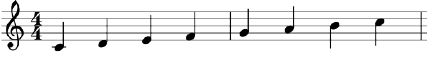
\includegraphics[width=10cm]{..//resources//images//partitura.JPG}
    \caption{Scara ascendentă C major în notația prin partitură \cite{Generating-Guitar-Tablatures-with-Neural-Networks}.}
\end{figure}

Acest model de prezentare a notelor muzicale este format dintr-un 
grilaj cu 5 linii, pe care sunt organizate notele. O notă 
poate să fie localizată fie pe o linie, fie între două 
linii. Este important de precizat faptul că această structură 
corespunde cu aspectul tastaturii unui pian, dar nu are o 
legătură directă cu modul în care sunt organizate notele 
în compunerea acordurilor pentru chitară \cite{Generating-Guitar-Tablatures-with-Neural-Networks}. 
Pentru a exemplifica 
dispunerea notelor în scară, pentru notația prin partitură,
Figura 2.2 exemplică toate notele muzicale într-o octavă, 
pornind de la nota C fundamentală. Cu acest reguli stabilite,
un fragment de partitură este prezentat în Figura 2.2.

\begin{figure}[h!]
    \centering
    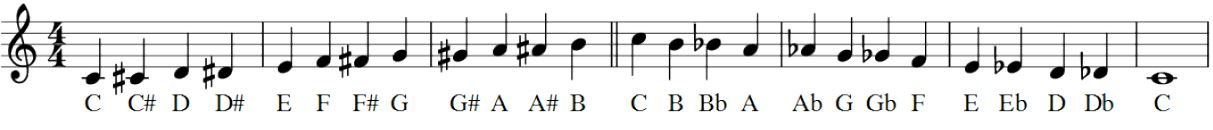
\includegraphics[width=15.8cm]{..//resources//images//partitura_2.JPG}
    \caption{Exemplificarea notelor muzicale într-o octavă, în notația 
    prin partitură \cite{Generating-Guitar-Tablatures-with-Neural-Networks}.}
    \label{}
\end{figure}

Aceste notații stau la baza reprezentării muzicale pentru notația prin partitură.
Există foarte multe alte notații, cu diferite definiții, înțelegerea și 
utilizarea lor fiind dependentă de studiul aprofundat al teoriei muzicale. 
Prin urmare, acest tip de notație nu este dedicat în mod special publicului 
larg, cu precădere interpreților de muzică acustică la chitară, pentru 
care acest tip de reprezentare a notelor muzicale nu este sugestiv.

\newpage
\section{Tabulatura}
Notația prin partitură descrie conținutul muzical, astfel poate să fie 
utilă și pentru a da diverse 
instrucțiuni directe despre cum trebuie abordată o piesă.
Prin comparație, tabulatura surprinde la rândul ei 
aceste instrucțiuni și este deosebit de populară în rândul 
chitariștilor amatori și experimentați, prin faptul că sunt simple 
și eficiente pentru a fi citite sau scrise \cite{Generating-Guitar-Tablatures-with-Neural-Networks}.

O tabulatură este formată din 6 linii orizontale care simbolizează 
corzile unei chitări, unde linia cel mai de sus corespunde cu cea mai de 
jos (cea mai subțire) coardă de pe chitară.
Cifrele care apar pe tabulatură reprezintă fretul (tasta) care 
trebuie atinsă pentru a cânta o anumită notă. Cifra 0 sugerează 
faptul că acea coardă trebuie atinsă în mod liber, fără a apăsa 
pe niciun fret cu degetul, lăsând coarda să sune liber. Dacă 
cifrele stau pe aceeași poziție verticală în tabulatură, atunci acele 
note trebuie cântate concomitent \cite{WEBSITE:tabulaturi}. 
Un fragment de tabulatură muzicală este prezentat în Figura 2.3.

\begin{figure}[h!]
    \centering
    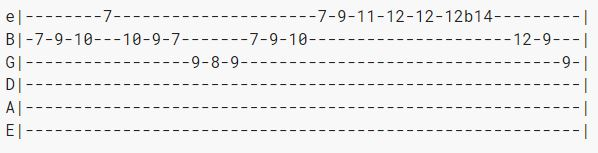
\includegraphics[width=12cm]{..//resources//images//tabulatura.JPG}
    \caption{Fragment de tabulatură din piesa 
    "And Your Bird Can Sing", The Beatles \cite{WEBSITE:ultimate-guitar}.}
    \label{}
\end{figure}

Astfel, tabulatura este extrem de folositoare pentru a exprima 
relația dintre note și chitară, mai precis, dintre note și 
corzile unei chitări, prin specificarea poziției exacte.
Acest tip de specificare este util în momentul în care sunt mai multe 
note care trebuie cântate consecutiv, într-un interval scurt de timp. 
Dacă este vorba de o interpretare acustică bazată pe acorduri muzicale, 
atunci se preferă reprezentarea fiecărui acord în parte, printr-o tabulatură
puțin modificată. Acest tip de reprezentare este concentrată pe descrierea 
fiecărui acord în parte, prin specificare fret-urilor, dar și a degetelor 
care trebuie folosite pentru realizarea acordului. 

Specificarea unui 
acord clasic (Em) este prezentată în Figura 2.4. Aceste reprezentări se 
vor folosi și pentru aplicația mobile, pentru a marca fiecare acord 
recunoscut de către sistem.

\begin{figure}[h!]
    \centering
    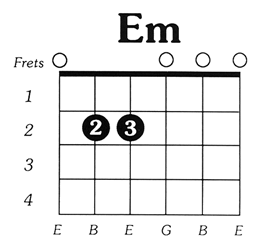
\includegraphics[width=3.5cm]{..//resources//images//em.png}
    \caption{Specificarea acordului Em. Se apasă cele două corzi marcate 
    utilizând degetul 2 (mijlociu) și degetul 3 (inelar) \cite{WEBSITE:guitar-chords-chart}.}
    \label{}
\end{figure}

\chapter{Metode de procesare ale semnalului sonor}
În acest capitol sunt prezentate diferite metode de procesare low-level a semnalului sonor, 
cu scopul obținerii unor caracteristici și a unei reprezentări care va fi utilizată mai departe în 
definirea și antrenarea unui model neuronal, prin învățare automată.
\section{Semnalul sonor}
Sunetul, prin definiție \cite{Audio-Sig-Processing}, este un semnal de tip mono-dimensional, 
dependent de timp, 
reprezentând presiunea aerului asupra canalului uman auditiv. Sistemul auditiv uman 
este capabil să perceapă orice semnal sonor care se află în intervalul de frecvență 
20Hz - 20000Hz (=20kHz).

Frecvența se definește ca numărul de repetări ale unui fenomen sau eveniment periodic 
într-un interval de timp. Unitatea de măsură pentru frecvență este Hertz, simbolizat 
ca Hz, denumită astfel în cinstea fizicianului german Heinrich Hertz. Astfel, o 
frecvență f = 1 Hz este corespunzătoare unei perioade de timp de o secundă.

Putem astfel afirma că dacă un anumit eveniment se repetă la un interval de timp T, putem 
calcula frecvența f ca:
\begin{equation*}
    f = \frac{1}{T}\
\end{equation*}

In ceea ce privește sunetul, frecvența este legată de noțiunea de înălțime muzicală.
Astfel, pentru nota LA din gama centrală se definește frecvența de 440 Hz, ceea ce 
înseamnă că aerul pus în mișcare de unda sonoră corespunzătoare oscilează de 440 de 
ori pe secundă.

Sunetul capturat de către un microfon este o undă dependentă de timp, determinând 
variația presiunii aerului în câmpul sonor în care se află microfonul. Astfel, 
un semnal audio digital este obținut prin prelevarea și cuantificarea adecvată 
a ieșirii microfonului, reprezentat de unde electice. Deși orice frecvență 
peste 40kHz ar fi suficientă pentru a capta întreaga gamă de frecvențe perceptibile, 
rata de preluare utilizată pe o scară largă este de 44.100 Hz, stabilită în urma 
nevoii de a sincroniza sunetul cu datele de tip video.

Calitatea de tip \emph{CD} se referă la o mostră audio digitală cu frecvența de 44.1 kHz 
și 16-bit (adâncimea de biți sau \emph{bit depth}, reprezintă numărul de biți de informație 
aflați în fiecare mostră audio).

Pentru a înțelege mai bine calitatea sunetului în funcție de adâncimea de biți 
observăm Figura 3.1, unde se prezintă prin comparație forma undei în funcție de valoarea
adâncimii de biți.
\begin{figure}[h!]
    \centering
    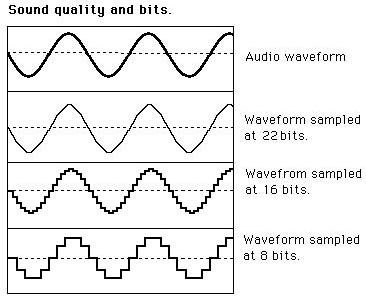
\includegraphics[width=8cm]{..//resources//images//bits_ex.jpg}
    \caption{Calitatea undei sonore în funcție de adâncimea de biți \cite{WEBSITE:victorimpmooc}. 
    Pe primul rând se observă unda sonoră originală, având 24 biți.}
    \label{fig:bits}
\end{figure}

Prin intensitate sonoră se înțelege senzația produsă de amplitudinea unei unde 
sonore, cunoscută și ca volumul vibrației, asupra organului uman auditiv. Cu cât amplitudinea este 
mai mare, cu atât crește și intensitatea sunetului care rezultă. Intensitatea sonoră 
se măsoară în unități denumite în fizică decibeli (dB) sau foni (un decibel este 
echivalent cu un fon).

Auzul uman este limitat de un interval în ceea ce privește intensitatea sunetului, 
și anume:
\begin{enumerate} 
    \item Marginea inferioară:
    \begin{itemize} 
        \setlength\itemsep{0.2em}
        \item prag auditiv cu valoarea de 0 dB;
        \item sunete foarte slabe ca intesitate, cum ar fi: sunete din natură, nivelul de zgomot 
        dintr-o bibliotecă, cu valoarea cuprinsă între 10-20 dB.
    \end{itemize}
    \item Marginea superioară:
    \begin{itemize} 
        \setlength\itemsep{0.2em}
        \item sunete extrem de puternice ca intensitate, cum ar fi: decolarea unui avion cu reacție, 
        cu valoarea cuprinsă între 120-130 dB;
        \item prag dureros cu valoarea de 140 dB \cite{Ed-muz-sinteze-corelari-interdisc}.
    \end{itemize}
\end{enumerate}
\section{Transformata Fourier pe termen scurt}
Pentru a putea înțelege metoda transformatei fourier pe termen scurt, 
este nevoie de definirea bazelor matematice ale Transformatei Fourier (FT) și procesele care compun 
metoda.

\subsection{Interpretare matematică}
Se consideră, drept exemplu, un semnal pur cu frecvența \emph{f} de 3Hz, 
pe un interval de timp vizibil. (Figura 3.2)

\begin{figure}[h!]
    \centering
    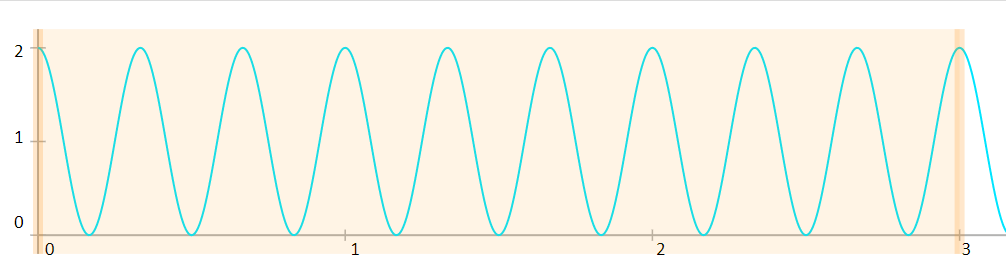
\includegraphics[width=12cm]{..//resources//images//semnal_3hz.png}
    \caption{Undă sonoră cu frecvența de 3Hz \cite{WEBSITE:fourier-visualization}.}
    \label{fig:bits}
\end{figure}

Se transpune această undă dependentă de timp în jurul unui cerc prin intermediul unei
corzi, în așa fel încât valorile extreme ale funcției din prima reprezentare 
să fie asociate cu distanțele maxime în raport cu originea din cea de-a doua 
reprezentare. De aici se observă că trebuie luată în considerare o nouă frecvență, și anume frecvența de realizarea a unui 
rotații complete de cerc parcurgând coarda, notată \emph{fcerc}. 

\iffalse
\begin{figure}[h!]
    \centering
    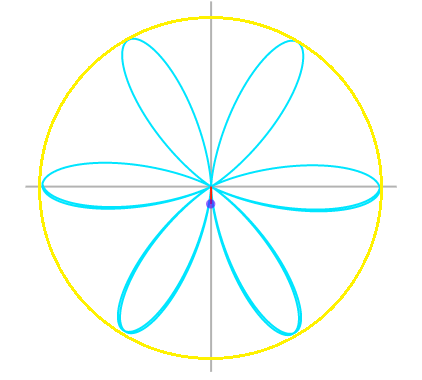
\includegraphics[width=4cm]{..//resources//images//fourier_cerc.png}
    \caption{Reprezentarea undei sonore în jurul unui cerc prin intermediul unei corzi, 
    cu \emph{fcerc} = 0.5 rotații/sec. \cite{WEBSITE:fourier-visualization}.}
    \label{fig:bits}
\end{figure}
\fi

\iffalse
Această frecvență poate fi ajustată în orice 
fel, dar valoarea ei influențează modul în care se ondula coarda 
în reprezentarea a doua.
\fi

Se presupune că această coardă are o masă și se consideră punctul central ca 
fiind \emph{centrul de masă} al corzii. Se observă că odată cu modificare frecvenței cerc, 
se modifică și poziția centrului de masă, care se situează într-o vecinătate restrânsă 
a originii, cu o singură excepție: momentul în care frecvența de realizare a unei rotații în jurul
cercului, \emph{fcerc}, este egală cu frecvența undei sonore, notată \emph{f}.

\iffalse
În această situație centrul de masă se depărtează de origine, sugerând un decalaj pentru aceea valoare
a frecvenței. Pentru a urmări mișcările centrului de masă în raport cu originea, dar și eventualele decalaje, 
se poate realiza un grafic timp-decalaj, grafic care se va apropia conceptual de reprezentarea fourier
a undei sonore. (Figura 4)

\begin{figure}[h!]
    \centering
    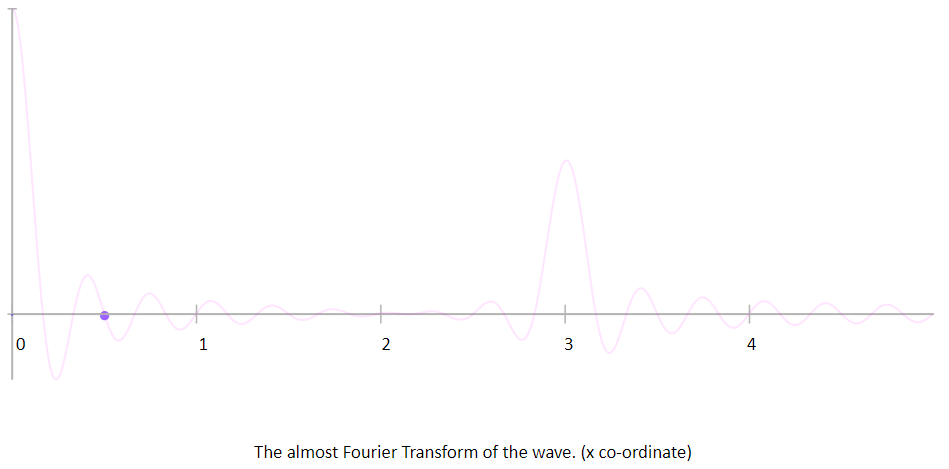
\includegraphics[width=12cm]{resources//images//almost-fourier.png}
    \caption{Centrul de masă, raportat la origine \cite{WEBSITE:fourier-visualization}}
    \label{fig:bits}
\end{figure}
\fi

Punctul specific centrului de masă poate fi reprezentat sub forma unui număr complex de forma $xi + yj$.
Se alege o reprezentare de tip complex în detrimentul unei reprezentări standard în coordonate $(x,y)$
deoarece numerele complexe oferă o descriere potrivită pentru rotiri și ondulări raportate la un cerc de rază, notat $r$.
De exemplu, formula lui Euler, una dintre cele mai faimoase formule trigonometrice($e^x = cos(x) + isin(x)$),
enunță faptul că $e^{ix}$ trasează cercul unitate din planul numerelor complexe, când x ia valori reale.
\iffalse
Astfel, dacă \emph{fcerc} = 1 rotații/sec, rezultă expresia $e^{2{\pi}ift}$, unde 
\emph{t} reprezintă intervalul de timp, iar \emph{f} reprezintă frecvența.
\fi 
Astfel, dacă \emph{f=1/10}, atunci
o rotație completă se va realiza odată la 10 secunde.
De asemenea, convenția în cadrul transformatei Fourier este ca rotația să se realizeze în jurul
acelor de ceasornic, expresia devenind $e^{-2{\pi}ift}$.

Fie o funcție $g(t)$ ce descrie un semnal dependent de intensitate și timp. Dacă se înmulțește
$g(t)$ cu expresia construită, punctul din planul complex se va plimba de sus în jos potrivit
valorilor funcției $g(t)$. Astfel, expresia $g(t) e^{-2{\pi}ift}$ încapsulează întreaga idee de 
ondulare a funcției g în jurul unui cerc cu o variabilă pentru frecvența $f$.  

Totuși, scopul este de a urmări mișcarea centrului de masă pe care îl are coarda. Pentru 
a aproxima centrul de masă pot fi considerate mai multe \emph{mostre} din semnalul original reprezentat 
de funcția g, apoi urmărite pozițiile lor în reprezentarea din jurul cercului, și realizată o medie.
Cu cât se iau în considerare mai multe puncte, cu atât rezultatul va fi mai precis. Generalizând, se consideră
o integrală a acestei funcții.
\iffalse
\begin{equation*}
    \int_{t1}^{t2} g(x) e ^ {-2 {\pi}i fx} dx
\end{equation*}
\fi
De la această integrală până la transformata Fourier mai este un singur pas, și anume trebuie considerată
integrala de tip continuu, pe intervalul $(-\infty, \infty)$. Astfel, formula este următoarea:
\begin{equation*}
    F(\epsilon) = \int_{-\infty}^{\infty} f(x) \cdot e ^ {-2 {\pi}i {\epsilon} x} dx
\end{equation*}

O proprietate importantă este forma continuă a tranformatei, 
întrucât integrala este definită pe intervalul de timp $(-\infty, \infty)$. În practică însă, 
colectarea de date audio se realizează într-un interval 
finit de timp (de la momentul de start $t_0$ la momentul $t_N-1$), ceea ce 
implică calculul unei transformate de tip discret, \emph{Discret Fourier Tranform} (DFT). 

Transformata de tip discret are aceeași definiție ca transformata de tip continuu, 
diferența fiind doar în stabilirea unui interval finit cunoscut, calcul integralei 
fiind înlocuit de o sumă finită care are următoarea formă:
\begin{equation*}
    X({\epsilon}_k) = \sum_{n=0}^{N-1} f(t_n) \cdot e ^ {-2 {\pi}{\epsilon}_k t_n } , k = 0,1,2...,N-1
\end{equation*}

Semnificația fiecărei variabile din formulă este următoarea:
\begin{itemize} 
    \setlength\itemsep{0.2em}
    \item f($t_n$), semnalul de intrare, la momentul n;
    \item $X(\epsilon_k)$, valoarea complexă a spectrului corespunzător lui x, la frecvența k;
    \item N, totalul semnalelor de intrare (mostre);
    \item $t_n = nT$, unde T reprezintă intervalul de eșantionare a semnalului, fiind măsurat în 
    secunde și n, o valoare de tip întreg, $n>=0$;
    \item $f_s = \frac{1}{T}$, reprezentând rata de eșantionare, măsurată în Hz; 1Hz = 10000 de 
    eșantioane pe secundă \emph{(samples per second)};
    \item $\epsilon_k = k\Omega$, este al k-lea eșantion din totalul mostrelor de intrare;
    \item $\Omega = \frac{2{\pi}}{NT}$, interval de eșantionare cu frecvența radiană, rad/sec \cite{Bonvini-Recognition}.
\end{itemize}

În literatură se obișnuiește ca T să fie egal cu 1 în ecuația precedentă și astfel se 
obține $t_n = n$. Atât semnalul $x(n)$ cât și transformarea $X(\epsilon_k)$ sunt cantități
discrete reprezentând N mostre. 
\iffalse
Dacă se notează în ecuația precedentă:
\begin{equation}
    s_k(n) = e^{-2 {\pi}{\epsilon}_n n} 
\end{equation}
aceasta poate fi rescrisă astfel:
\begin{equation}
    X({\epsilon}_k) = <x, s_k>
\end{equation}
Astfel, transformarea poate fi văzută ca o măsură a similarității dintre un semnal 
$x(n)$ și o exponențială complexă $s_k(n)$. 
\fi
Semnalul audio este foarte non-staționar. 
Dezavantajul metodei DFT este că informația temporală \emph{(temporal information)} se pierde.
Din acest motiv, este necesar să se compună o analiză locală a frecvenței pe secțiuni și nu
luând semnalul întreg \cite{Bonvini-Recognition}. 
Această metodă se numește \emph{Transformata Fourier pe termen scurt (STFT)}. 
Procesul este ușor de realizat calculând DFT pe porțiuni ale semnalului, numite
cadre. Parametrii care trebuie specificați sunt:
\begin{itemize}
    \setlength\itemsep{0.2em}
    \item $N_{FT}$, dimensiunea totată a semnalului;
    \item $L, L <= N_{FT}$, dimensiunea unui cadru din semnal;
    \item saltul \emph{(hop size)}, notat $Hop$, reprezentând distanța în eșantioane între 
două cadre consecutive.
\end{itemize}

Astfel, formula de calcul pentru STFT este următoarea:
\begin{equation*}
    X_{stft}({\epsilon}_k, r) = \sum_{n=0}^{N_{FT}-1} (x(n - rHop){\epsilon}_n) e ^ {-2 {\pi}{\epsilon}_k n } , k = 0,1,2...,N_{FT}
\end{equation*}

\subsection{Aplicabilitate}
Transformata Fourier este o un tip de operație care se aplică unei 
funcții complexe și produce o altă funcție complexă care conține aceeași informație ca funcția originală, 
dar reorganizată dupa frecvențele componentelor.

Se dorește ca, utilizând principiile matematice ale transformatei Fourier 
enunțate mai sus, să se găsească o reprezentare
a undei sonore, pe baza căreia se pot extrage caracteristici utile, aplicând transformata Fourier sau orice altă
metodă derivată.
Astfel, se consideră o funcție reprezentată de un semnal dependent
de timp, care este chiar unda sonoră, dar limitată la un interval temporal. 
Transformata Fourier a funcției descompune semnalul după frecvență și 
produce un spectru al acestuia.

Proprietatea de bază a transformatei este dată de reorganizarea informației 
după frecvențe (temporale, spațiale sau de alt fel), 
fiind extrem de utilă în prelucrarea semnalelor de diverse tipuri, 
în înțelegerea propriețăților unui număr mare de sisteme fizice sau 
în rezolvarea unor ecuații și sisteme de ecuații \cite{Fourier-Transform}.
De asemenea, transformata Fourier permite analiza semnalului și identificarea anumite
frecvențe dorite, cu scopul de a le amplifica sau a le suprima, și astfel, determinându-se sintetizarea unui
nou semnal. 

Înzestrată cu aceste propietăți, dar și cu altele, transformata este 
prezentă în foarte multe tehnologii și domenii moderne (ultimul domeniu în care și-a găsit aplicabilitea 
fiind mecanica cuantică), deoarece este mai fiabilă și mai robustă decât alte tehnologii de analiză
a semnalului de orice fel și compunere a spectrului.

Dezavantajul principal constă în dificultatea și complexitatea 
calculelor care determină întregul proces. În cazul integrării transformatei
într-un program soft, programatorul trebuie să transpună procesul 
într-un algoritm eficient și să fie conștient de faptul că unele calcule
utilizează procesoarele într-un mod intens.

La nivelul limbajelor de nivel înalt, cum ar fi Python, există librării care vin în
ajutorul programatorilor cu metode de procesare audio implementate într-un mod eficient(de exemplu, utilizarea
librăriei LibROSA).

\iffalse
Studiul transformatei Fourier pornește de la studiul seriilor Fourier, fiind folosite  
pentru a analiza funcții periodice complexe și pentru a le descompune ca sume 
ponderate de unde matematice reprezentate de funcțiile sinus și cosinus. 
Propietățile acestor funcții ne permit să revenim la valorea fiecarei unde 
prin intermediul unei integrale.
\fi

\newpage
\section{Transformata Q constantă}
Principala problemă în aplicarea Transformatei Fourier în aplicații muzicale este faptul că intervalele
de eșantionare ale frecvenței pentru o mostră muzicală sunt liniar distribuite, acest aspect fiind diferit
în cadrul transformatei Q constantă, unde intervalele sunt distanțate în mod geometric.

Transformarea Q constantă (CQT) a fost introdusă de Brown în \cite{Constant-Q-Spectral} și este 
asemănătoare transformatei Fourier.
Utilitatea acestei 
transformări se bazează pe faptul că, având un mod adecvat de alegere a parametrilor, 
frecvențele $f_k$ ale transformării vor corespunde
în mod direct cu cele ale notelor muzicale. Frecvențele corespunzătoare se determină
astfel prin formula:

\begin{equation*}
    f_k = f_0 \cdot 2 ^ { \frac{k}{{\beta}}\ }, k=0,1,...
\end{equation*} 
unde, k reprezintă a k-a frecvență, $f_0$ corespunde celei mai mici frecvențe iar $\beta$
reprezintă numărul de filtre dintr-o octavă. 
\iffalse
Astfel, formula devine:
\begin{equation*}
    X_{cq}(k,r) = \frac{1}{N_k}\ \sum_{n <= N_k}^{} x(n-rHop){\omega(n)}e^{j2{\pi}nQ/{N_k}}, 
\end{equation*} 
unde $Q = (2 ^ \frac{1}{\beta}\ - 1)^ {-1}$ și $N_k = [Q \frac{f_s}{f_k}]$.
\fi

De asemenea, valoarea pentru rezoluția în domeniul timp a
transformatei Q, \emph{time resolution}, crește odată cu creșterea frecvenței. Acest aspect
este similar cu comportamentul sistemului uman auditiv \cite{Bonvini-Recognition}. 
Concluzia acestei proprietății este că atât simțul uman auditiv, cât și computerul digital, au
nevoie de mai mult timp pentru a percepe frecvența unui ton muzical scăzut.

Metoda nu este foarte eficientă în ceea ce privește timpul total de compunere a 
frecvențelor și de determinare a reprezentări, dar reprezintă o optimizarea a
tranformatei Fourier clasice, fiind utilizată pe o scară mai largă, prin aplicarea
diverselor strategii de calcul paralel pentru a scădea timpul de execuție, în cazul
în care transformata este aplicată pe un set de date numeros.

Librăria LibROSA oferă o soluție eficientă și ușor 
de utilizat pentru calculul transformatei Q constantă a unui semnal audio, fiind nevoie doar 
de încărcarea semnalului și de cunoașterea parametriilor ca \emph{hop length}, reprezentând 
valoare pentru salt, și opțional, \emph{n{\_}chroma}, pentru a specifica numărul de semitonuri 
distincte dorite pentru octava muzicală (implicit, valoarea pentru acest 
parametru este 12). Astfel, o metodă simplă de calcul arată astfel:

\begin{python}

    def compute_chroma_cqt(audio_file_path):
        #   Se incarca fisierul audio folosind sistemul de incarcare 
        # oferit de LibROSA
        audio, sr = librosa.load(audio_file_path)
        #   Determina chromagrama folosind transformarea Q constanta 
        chromagram = librosa.feature.
                chroma_cqt(audio, sr=sr, hop_length=512, n_chroma=24)
\end{python}

\iffalse
Brown a propus \cite{Constant-Q-Spectral} un algoritm mai eficient
bazat pe inmulțiri de matrici bazate în domeniul frecvențelor. Formula de calcul care
stă la baza algoritmului optimizat este:    

\begin{equation*}
    X_{cq} = \frac{1}{N} X_{stft} S
\end{equation*}

unde, $X_{stft}$ reprezintă transformata fourier pe termen scurt a semnalului $x(n)$ iar 
S reprezintă trasformarea fourier rapidă (FFT - o altă metodă de transformare ce are la 
bază tot transformata Fourier). 
\fi

\newpage
\section{Chromagrama}
Chromagrama este reprezentarea unui grup de caracteristici pe care un program ce are la 
bază unul din algoritmii de procesare audio, îl extrage dintr-un semnal audio. Reprezentarea 
este bazată pe profilul notelor rădăcină, cunoscut ca \emph{pitch class profile (PCP)}, acesta 
fiind un descriptor în contextul unui sistem de recunoaștere a acordurilor. 

Chromagrama este formată astfel dintr-o secvență de vectori caracteristici, fiecare având 
rolul de a măsura intensitatea relativă a fiecărei note, raportată la fiecare frame, într-un interval 
de timp. Se obține astfel o diagramă de tipul pitch class versus time, adică o imagine 
a semnalului audio, ce conține informații concludente, care pot ajuta în determinarea celui 
mai probabil acord.

\iffalse
Scopul chromagramei, cunoscută și ca \emph{pitch class profile(PCP)}, 
este să scoată în evidență contribuția pe care o are fiecare sunet/notă, 
\emph{pitch class}, raportat la energia care se găsește în fiecare frame, într-un interval de timp.
Ca rezultat, se obține o reprezentare pitch class versus timp pe baza semnalului de intrare.
În acest fel, informația obținută poate fi folosită în mod direct pentru a găsi cel mai posibil
acord care se cântă în acel moment.
\fi

În literatură există diferite metode de a construi o chromagramă. Principalii pași 
enunțati de către Bello si Pickens în \cite{Harmonic-content-in-music-signals},
vor fi folosiți ca bază de lucru și în procesele acestui algoritm. Pașii pentru compunerea 
chromagramei sunt următorii:
\begin{itemize}
    \setlength\itemsep{0.2em}
    \item Convertirea semnalului audio într-o reprezentare intermediară, numită spectogramă, 
    prin aplicarea unei transformări Fourier derivată sau optimizată;
    \item Se aplică un filtru asupra frecvențelor din cadrul spectogramei, pentru a se încadra în 
    intervalul 100Hz - 5000Hz;
    \item Se construiește profilul notelor rădăcină, pe baza frecvențelor estimate. Este o procedură pentru 
    a determina nota rădăcina \emph{(pitch class)}, din valorile frecvențelor;
    \item Se realizează o normalizare a caracteristicilor, cadru cu cadru, prin divizarea cu cea mai 
    mare valoare, pentru a elimina zgomotul, rezultând imaginea chromagramei. Figura 3.3 prezintă 
    chromagrama obținută prin aplicarea pașilor asupra unui acord muzical. 
\end{itemize}
\begin{figure}[h!]
    \centering
    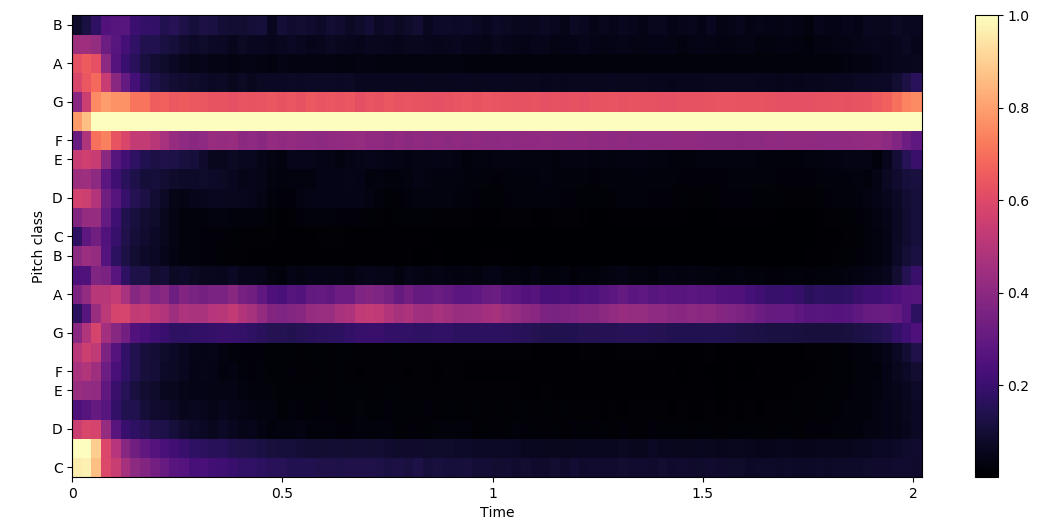
\includegraphics[width=13.2cm]{..//resources//images//Chroma_Am.png} 
    \caption{Imaginea obținută prin construirea chromagramei acordului A, reprezentare grafică 
    utilizând LibROSA și matplot. }
    \label{fig:bits}
\end{figure}


\newpage
\chapter{Metode de clasificare}
\section{Sisteme de învățare automată}
Învățarea automată \emph{(machine learning)}, este o ramură a Inteligenței 
Artificiale concentrată pe algoritmi specializați pe invățarea din date. 
Procesul de învățare constă în deducerea unor tipare, pe baza unor reguli
bine stabilite. Mai precis, se urmărește crearea unui program complex capabil 
să generalizeze un comportament indiferent de datele de intrare. 

Problemele clasice de învățare automată includ clasificare de imagini sau de înregistrări 
audio, recunoaștere vocală, evaluarea riscurilor financiare pentru 
diverse investiții, dezvoltarea unor strategii în jocuri sau simulări, predicția unor
diagnostice medicale etc. 
În mod general, abordările algorimilor sunt structurate după obiectivul 
lor de învățare: 
\begin{enumerate}
    \item Învățare supervizată \\ În cadrul învățării supervizate, datele de antrenament care alimentează algoritmul 
    includ predicția corectă, numite etichete, sau \emph{labels}. Un exemplu de metodă clasică
    este \emph{metoda clasificării}. O problemă clasică care are la bază clasificarea este 
    problema filter-ului de email-uri spam. Aici antrenarea se realizează cu multe exemple
    de email-uri, fiecare din ele având clasa corespunzătoare atașată (spam sau not-spam).
    Astfel, modelul va învăța cum să clasifice orice mail nou întâlnit \cite{Hands-On-Machine-Learning}. \\
    O altă metodă specifică este \emph{metoda regresiei}. Problemele de regresie au ca scop prezicerea unei valori numerice
    target, pe baza unor trăsături numite predictori (de exemplu, prezicerea prețului pentru o mașină
    pe baza unor trăsături ca marca, anul de fabricație și distanța parcursă). 
    Pentru a se realiza antrenarea, este necesară utilizarea unui set de predictori împreună cu etichetele 
    corespunzătoare.\\
    Cei mai importanți algoritmi de învățare supervizată sunt următorii:
        \begin{itemize} 
            \item Cei mai apropiați k vecini;
            \item Modele Markov cu stări ascunse (HMMs) - \emph{statistical learning}
            \item Regresie liniară;
            \item Regresie logistică; 
            \item Mașini cu suport vectorial (SVMs);
            \item Arbori de decizie;
            \item Rețele neuronale artificiale.
            \item Rețele neuronale profunde (CNNs, DBNs) \cite{Hands-On-Machine-Learning}.
        \end{itemize}
    \item Învățare nesupervizată: \\ În cadrul învățării nesupervizate datele utilizate pentru antrenament 
    nu sunt etichetate. Astfel, în funcție de date și de domeniul problemei, algoritmii sunt împărțiți în
    subcategorii, după cum urmează:
    \begin{enumerate}
        \item Clustering: se definește ca un proces de organizare a obiectelor asemănătoare dintr-un anumit punct de vedere. Astfel, noțiunea de \emph{cluster} definește
        o mulțime de obiecte similare între ele și diferite de obiectele care aparțin altui cluster. Pentru exemplificare, 
        se consideră o problemă care dorește împărțirea pe clustere a vizitatorilor unui blog. În niciun moment
        dezvoltatorul sistemului nu va interveni pentru a ajuta algoritmul cu informații despre vizitatori. Conexiunile
        între utilizatori vor fi determinate în mod independent de către algoritm \cite{Hands-On-Machine-Learning}. \\ Spre exemplu, se poate observa
        că 30\% dintre utilizatori sunt bărbați care sunt pasionați de carți polițiste și în general citesc blog-ul
        în jurul amiezei, în timp ce 20\% sunt tineri pasionați de sci-fi si citesc blog-ul în weekend etc. Astfel,
        dacă se utilizează un algoritm de clustering bazat pe ierarhii, \emph{hierarchical clustering}, se pot realiza
        subdiviziuni pe baza acestor informații care pot ajuta la distribuirea ulterioară în clustere. 
        Figura 4.1 prezintă un grafic general care abordează problema grupării datelor în clustere.

        \begin{figure}[h!]
            \centering
            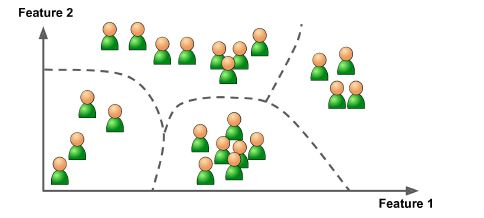
\includegraphics[width=10cm]{..//resources//images//clustering.jpg}
            \caption{Abordarea generală a grupării în clustere \cite{Hands-On-Machine-Learning}.}
        \end{figure}
        Cei mai cunoscuți algorimi de clustering sunt: \emph{K-Means}, \emph{Hierarchical clustering} și 
        \emph{Clustering bazat pe densitatea aplicațiilor cu zgomot (DBSCAN)}.
        \item Vizualizarea și reducerea dimensionalității: algoritmii de vizualizare se definesc ca algoritmi 
        care se încarcă cu numeroase date, iar pe baza lor se obține ca output un grafic 2D sau 3D ca
        reprezentare a datelor, cu scopul de a înțelege cum sunt organizate acestea, cu posibilitatea descoperirii
        unor modele neașteptate. O sarcină conexă este reducerea dimensionalității, în care obiectivul este simplificarea
        datelor fără a pierde multe informații. \\
        Spre exemplu, distanța parcursă de o mașină poate fi corelată
        cu vârsta sa, astfel algoritmul de reducere va îmbina cele două caracteristici într-o singură 
        caracteristică ce reprezintă uzura mașinii. \\
        Printre cele mai utilizate metode se numără: \emph{Analiza componentelor principale (PCA)},
        \emph{Kernel PCA}, \emph{Încorporarea linear locală (LLE)} \cite{Hands-On-Machine-Learning}. 
        \item Reguli de asociere: învățarea prin intermediul regulilor de asociere are ca scop analiza
        cantităților mari de date și descoperirea relațiilor interesante între atribute. \\
        De exemplu, să presupunem că deținem un supermarket. Efectuarea unei reguli de asociere pe
        jurnalele de vânzări dezvăluie faptul că persoanele care cumpără sos de friptură și cartofi,
        tind să cumpere și friptură. Astfel, este de dorit ca articolele de acest tip să fie plasate aproape
        unele de altele. \\
        Printre algoritmii cei mai utilizați se numără: \emph{Apriori} și \emph{Eclat} \cite{Hands-On-Machine-Learning}. 
    \end{enumerate}
    \item Învățare semi-supervizată \\
    Învățarea semi-supervizată urmărește definirea unor algoritmi de învățare care au date de antrenament
    doar parțial etichetate. În majoritatea cazurilor, datele neetichetate predomină în setul de date.
    În mare parte algoritmii sunt construiți prin combinarea algorimiilor de învățare supervizată și
    nesupervizată. \\ 
    Spre exemplu, una din metode, rețelele \emph{deep belief} au la bază componente nesupervizate
    numite mașini cu restricție Boltzmann, \emph{restricted Boltzmann machines} (RBMs), componente așezate sub
    forma unei stive în definirea modelului \cite{Hands-On-Machine-Learning}. RBM-urile sunt antrenate secvențial într-o manieră nesupravegheată,
    și apoi, întregul sistem este ajustat folosind tehnici de învățare supravegheată.
    \item Învățare prin întărire \\
    Învățarea prin întărire este o metodă diferită de cele enunțate anterior. Sistemul de învățare, numit agent,
    este capabil să observe mediul, să selecteze și să efectueze acțiuni, în urma cărora primește \emph{recompense}.
    (sau penalități, sub forma de recompense negative) \cite{Hands-On-Machine-Learning}.
    Acest mecanism obligă sistemul să învețe de la sine cea mai bună strategie, numită politică, pentru a obține cu timpul cele mai bune recompense. O politică
    definește ce acțiuni să aleagă agentul atunci când se află într-o situație nouă, necunoscută.
\end{enumerate}
\iffalse
\section{Regresie logistică}
    Regresia logistică este unul dintre algorimii de regresie care poate fi abordat și din  
    perspectiva unei metode de clasificare. Algoritmul este frecvent folosit pentru a estima probabilitatea
    ca o instanță să aparțină unei clase particulare(de exemplu, care este probabilitea ca un email
    să fie spam?). Dacă probabilitatea este mai mare de 50\%, atunci modelul precize că instanța aparține
    acelei clase(numită clasă "pozitivă" și etichetată cu valoarea 1), sau, altfel, se presupun că
    nu aparține(aparține clasei "negative" etichetată cu valoarea 0). Acest comportament îl face 
    un clasificator binar.

    Modelul prin regresie logistică se compune prin calculul unei sume ponderate a caracteristicilor de intrare
    (valorile de input) plus o valoare constantă numită \emph{bias}. Output-ul nu este reprezentat de rezultatul
    direct al calculului, ci de logistica rezultatului. Logistica, notată $\sigma()$ este determinată de o
    funcție de activare, care pentru această metodă se alege a fi funcția sigmoid. Funcția sigmoid 
    care transpune orice valoare în intervalul [0,1]. Matematic, se definește astfel:
    \begin{equation*}
        \sigma(t) = \frac{1}{1 + e ^ {-t}}
    \end{equation*}
    
    \begin{figure}[h!]
        \centering
        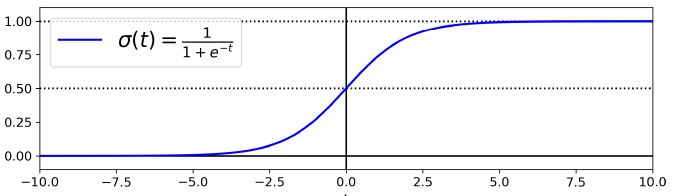
\includegraphics[width=12cm]{..//resources//images//sigmoid.jpg} 
        \caption{Reprezentarea funcției sigmoid \cite{Hands-On-Machine-Learning}.} 
    \end{figure}
    Odată ce modelul a estimat probabilitatea p ca o instanță să aparțina clasei considerate pozitive, se poate 
    calcula ușor predicția modelului: dacă p < 0.5, atunci instanța aparține clasei 0, altfel aparține clasei 1.
    Aceasta este metoda prin care algoritmul estimează probabilități și face predicții.

    Analiza mai complexă ține de modul în care acest model se antrenează. 
\fi
\section{Modele Markov cu stări ascunse}
Modelele Markov cu stări ascunse, \emph{Hidden Markov Models(HMM)}, se bazează pe determinarea 
unui lanț Markov. Un lanț Markov este un model care ne informează despre probabilitățile secvențelor
unor variabile aleatorii, numite stări, fiecare putând prelua valori din cadrul unui set. Aceste 
seturi pot reprezenta orice, de la cuvinte până la diverse simboluri (de exemplu, simboluri
care definesc vremea). 

Un lanț Markov face o presupunere foarte puternică în ceea ce privește prezicerea viitorului 
într-o succesiune, starea actuală fiind singura care contează. Stările anterioare stării curente
nu au niciun impact asupra previziunii din viitor. Spre exemplu, s-ar putea prezice vremea de mâine, 
examinând vremea de astăzi, fără a fi permisă analiza vremii de ieri.

\iffalse
\begin{figure}[h!]
    \centering
    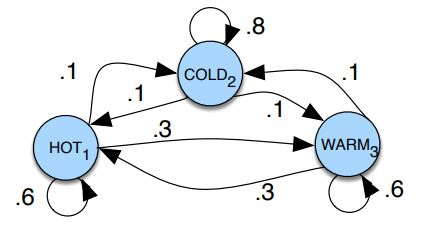
\includegraphics[width=10cm]{..//resources//images//hmm_chain.jpg} 
    \caption{HMM Chain}
\end{figure}
\fi

Astfel, fie o secvență de stări  $q_1,q_2,...q_i$. Un model Markov încorporează presupunerea Markov
în privința probabilităților acestei secvențe. Presupunerea Markov afirmă faptul că prezicerea
viitorului depinde doar de prezent, fără a conta trecutul. Matematic, se definește astfel:
    
\begin{equation*}
    P(q_i|q_1...q_{i-1}) = P(q_i|q_{i-1})
\end{equation*}

Un lanț Markov este util atunci când trebuie calculată o probabilitate pentru o secvență de 
evenimente observabile. În multe cazuri însă, evenimentele care sunt de interes sunt ascunse/invizibile 
și nu pot fi observate în mod direct. Un model Markov cu stări ascunse permite abordarea 
ambelor tipuri de evenimente, observabile și ascunse, considerate drept factori cauzali 
în modelul probabilistic. 

Modelele Markov cu stări ascunse sunt caracterizate de trei probleme fundamentale:
\begin{enumerate}
    \item Probabilitatea (\emph{Likelihood}): Fiind dat un HMM $\lambda = (A,B)$ și un set de observații O, 
    să se determine probabilitatea $P(O | \lambda)$;
    \item Decodarea (\emph{Decoding}): Fiind dat un set de observații O și un HMM $\lambda = (A,B)$
    să se determine cea mai bună secvență de stări ascunse Q;
    \\
    Cel mai comun algoritm de decodare este algoritmul lui Viterbi.
    Este un algoritm de programare dinamică pentru a găsi cea mai probabilă secvență de stări
    ascunse, numită calea Viterbi. Rezultatul este o succesiune de evenimente observate, mai 
    ales în contextul modelelor Markov cu stări ascunse.
    \item Învățarea (\emph{Learning}): Fiind dat un set de observații O și un set de stări 
    într-un HMM, să se determine prin învățare parametrii A și B.
    \\
    Algoritmul standard de antrenare a unui HMM este cunoscut ca \emph{forward-backward} sau 
    \emph{Baum-Welch algorithm}, fiind un caz special pentru algoritmul mai cunoscut, și anume
    \emph{Expectation-Maximization(EM)}. Algoritmul permite antrenarea atât a paramentrilor de tranziție (A), 
    cât și a celor de emisie (B). EM este un algoritm iterativ care calculează estimări inițiale
    pentru probabilități, apoi folosește aceste estimări pentru a calcula o estimare mai bună, procesul
    continuând în acest fel, îmbunătățind iterativ probabilitățile pe care le învață \cite{Speech-and-Language-Processing}.
    \\
    Structura clasică a unui model Markov este înfățisată în Figura 4.2.

\end{enumerate}

\begin{figure}[h!]
    \centering
    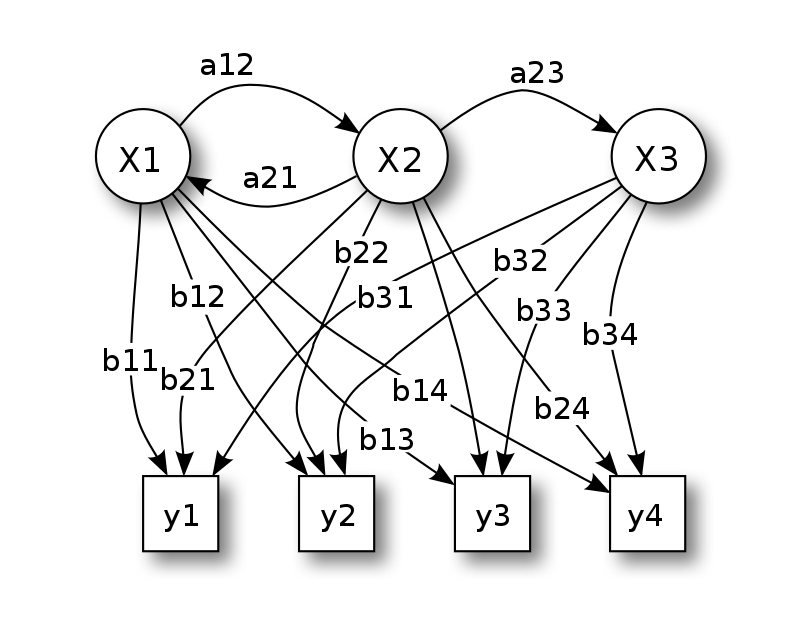
\includegraphics[width=10cm]{..//resources//images//hmm_model.png} 
    \caption{Model Markov cu stări ascunse, fiecare simbol reprezentând următoarele: X - stările, Y - posibilele observații, 
    a - probabilitățile de tranziție între stări, b - probabilitățile de emisie \cite{WEBSITE:hmm-model-figure}.}
\end{figure}

Pentru recunoaștere automată a acordurilor muzicale, se aplică problema de 
învățare a unui model Markov cu stări ascunse, utilizând pentru antrenare 
vectorii care determină reprezentarea prin chromagrama.
Modelul conține o singură stare pentru fiecare 
acord distins de către sistem. 

Astfel, cunoscându-se vectorii caracteristici observați (X), etichetele pentru acorduri (Q) 
și parametrii modelului curent ($\theta$), se poate calcula utilizând algoritmul EM
valoarea probabilității $P(X, Q|\theta)$ pe baza unei expresii definite ulterior. Algoritmul
garantează că estimările se vor îmbunătății de la o etapă la alta, ajungând
într-un optim local, în ceea ce privește setul de parametrii. Astfel, soluția estimează
în mod rezonabil un set de parametrii care maximizează probabilitea definită.

O astfel de abordare este descrisă în una din primele lucrări ștințifice ale domeniului,
despre care se va discuta în Capitolul 7. 

\newpage
\section{Rețele neuronale artificiale}
\emph{"Birds inspired us to fly, burdock plants inspired velcro, and countless more inventions
were inspired by nature. It seems only logical, then, to look at the brain’s architecture
for inspiration on how to build an intelligent machine \cite{Hands-On-Machine-Learning}."}

Creierul uman este cea mai complexă structură a corpului uman, fiind capabil de 
procesarea paralelă a informației, având o capacitate de stocare a ei de 85-100 de
miliarde de neuroni, fiecare având aproximativ 10000 de conexiuni.

Primul element care este astfel preluat de rețelele neuronale este neuronul. Neuronul 
este cea mai mică unitate fundamentală a sistemului nervos central, având rolul de a 
primi, conduce, procesa și transmite mai departe 
diferite semnale electrice primite de la organele 
de simț sau de la alți neuroni. Neuronul biologic este compus din \cite{Tehnici-de-inteligență-computațională-Aplicații-în-electronică-și-biomedicină}: 
\begin{itemize}
    \item Corp celular (Soma);
    \item Axon: având rolul de a transporta semnale către alți neuroni, sau celule țintă. Acesta 
are la capăt terminații sinaptice, prin care se poate lega cu dendritele altor neuroni sau direct
cu corpul lor;
    \item Dendrite: prin intermediul cărora se primesc semnale de la axonii altor neuroni;
    \item Sinapse: reprezintă conexiuni care se realizează între axonul unui neuron și 
dendritele altui neuron.
\end{itemize}

Preluând aceste informații biologice, se poate realiza o mapare a fiecărui element,
în vederea obținerii unei reprezentări pentru o rețea neuronală artificială. Această 
mapare poate fi observată în Tabelul 4.1.
\begin{table}[h!]
    \begin{center}
        \begin{tabular}{ | c | c | }
            \hline 
                RN Biologică  &  RN Artificială  \\
                \hline \hline 
                Soma  &  Nod  \\
                \hline
                Dendrite  &  Intrare  \\
                \hline
                Axon  &  Ieșire  \\
                \hline
                Activare  &  Procesare  \\
                \hline
                Sinapsă  &  Conexiune ponderată  \\
            \hline
        \end{tabular}
        \caption{Componente: rețea neuronală biologică vs. rețea neuronală artificială}
    \end{center}
\end{table}


Astfel, rețelele neuronale artificiale (ANN) se definesc ca structuri artificiale care
încearcă să reproducă modul de funcţionare a creierului uman. Sunt construite
din mai multe unități de procesare, numite și \emph{neuroni artificiali}, grupaţi în
straturi, fiecare strat având un număr diferit de elemente. 
Fiecare neuron poate primi informații de la alți neuroni, fiind acceptată 
chiar primirea de informații de la el însuși.  

Un neuron de tip artificial replică comportamentul unui neuron real. Astfel 
conexiunile dintre neuroni, cunoscute ca ponderi sinaptice, sunt folosite în
stocarea informației. După o procesare locală a semnalului de intrare pe baza 
informaţiei stocată în legăturile sinaptice (multiplicarea acesteia cu
valorile ponderilor stocate) se produce o sumare globală a
rezultatelor obţinute (proces similar cu cel ce are loc în corpul celular al
unui neuron biologic real). Dacă răspunsul rezultat depăşeşte un
anumit prag, informaţia este transmisă mai departe (utilizarea 
unei funcții de activare) \cite{Tehnici-de-inteligență-computațională-Aplicații-în-electronică-și-biomedicină}. 
Toate aceste elemente compun structura generală a unui neuron, care poate 
fi observată în Figura 4.3.

\begin{figure}[h!]
    \centering
    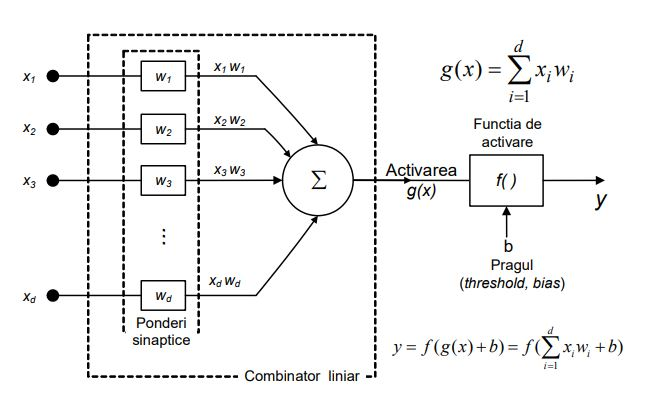
\includegraphics[width=13cm]{..//resources//images//structura_generala_a_unui_neuron.JPG} 
    \caption{Structura generală a unui neuron artificial \cite{Tehnici-de-inteligență-computațională-Aplicații-în-electronică-și-biomedicină}.}
\end{figure}

Valorile stocate în ponderi se schimbă prin intermediul 
algoritmilor de învățare. Astfel, în cadrul unui ANN, în general, cel care
construiește rețeaua nu trebuie să specifice valori pentru parametrii sistemului
(ponderile fiecărui neuron în parte). Valorile pentru acești parametrii vor fi extrase,
în mod automat, prin intermediul algoritmilor de antrenare sau adaptare. Fiecare algoritm se
clasifică în unul din obiectivele de învățare enunțate mai sus: supervizată, nesupervizată,
semisupervizată sau prin întărire.

Pașii care trebuie urmați pentru construirea 
unei rețele neuronale artificale sunt \cite{Hands-On-Machine-Learning}:
\begin{itemize}
    \item Construirea stratului de intrare cu m noduri;
    \item Constuirea stratului de ieșire cu n noduri;
    \item Determinarea numărului de staturi ascunse și construirea lor, cu unul sau mai mulți neuroni
    pe fiecare strat;
    \item Inițializarea ponderilor între nodurile aflate pe straturi diferite;
    \item Stabilirea funcției de activare corepunzătoare fiecărui neuron (de pe straturile ascunse).
\end{itemize}

Prin specificarea tutoror elementelor enunțate mai sus, se generează \emph{topologia} rețelei. Din punct
de vedere al topologiei, ANN-urile se clasifică în două tipuri:
\begin{itemize}
    \item Feed-Forward: Informația se propagă de la un strat la altul, de la intrare spre ieșire,
iar ieșirea fiecărui nod depinde de intrările sale care sunt conectate cu ieșirile neuronilor de pe 
stratul precendent. Sunt folosite în special pentru învățarea supervizată.
    \item Recurente: Prin intermediul legăturilor existente, se creează bucle ce determină ca 
ieșirea diferiților neuroni să fie dependentă și de valorile anterior calculate (spre exemplu, 
ieșirile altor neuroni de pe același strat). Au aplicabilitate atât pentru învățarea supervizată, cât
și pentru cea nesupervizată \cite{Tehnici-de-inteligență-computațională-Aplicații-în-electronică-și-biomedicină}.
\end{itemize}

Odată ce rețeaua a fost proiectată, procesul de antrenare (învățare) poate începe. Acest proces
urmărește obținerea unor valori optime pentru ponderile aflate între oricare două noduri ale 
rețelei, prin \emph{minimizarea erorii}. Eroarea se calculează determinând diferența dintre
rezultatul real și rezultatul calculat de rețea.

În general, rețelele neuronale artificiale sunt formate dintr-un număr mic de straturi (3-5),
cele mai frecvente fiind rețelele cu 3 straturi, adică cu un singur strat ascuns. Pentru 
construirea unor rețele mai complexe, nu se utiliează acest tip de rețele, fiind preferate
rețelele neuronale profunde (\emph{deep neural networks}). Această categorie de rețele 
utilizeză un număr superior de straturi, cu scopul de a dobândi capacitatea de a învăța 
reprezentări ale datelor de intrare cu nivele multiple de abstractizare (de exemplu, 
pentru clasificarea a milioane de imagini, recunoașterea audio, construirea unor
sisteme de recomandare audio/video sau înțelegerea limbajului natural).

\newpage
\section{Rețele neuronale profunde}
Nimic din natură sau din evoluția tehnologiei, până în ziua de azi, nu se compară cu abilitățile
complexe de procesare a informației și de recunoaștere a diferitelor modele complexe pe care 
le are creierul uman. Încercarea tehnologiei este a avansa în această direcție, dezvoltând 
algoritmi care imită rețeaua creierului uman, acestea fiind numite rețele neuronale profunde 
(\emph{deep neural networks}) \cite{WEBSITE:cnn-for-visual-recognition}.

Rețelele neuronale profunde au o structură unică, 
deoarece au o componentă ascunsă (formată din straturi ascunse) 
relativ mare și complexă între straturile de intrare și ieșire. 
Pentru a fi considerată o rețea neuronală profundă, 
această componentă ascunsă trebuie să conțină cel puțin două straturi \cite{Tehnici-de-inteligență-computațională-Aplicații-în-electronică-și-biomedicină}.
Datorită structurii lor, rețelele neuronale profunde au o capacitate 
mai mare de a recunoaște tipare decât rețelele superficiale.

Există câteva arhitecturi neuronale profunde consacrate, cum ar fi:
\begin{itemize}
    \item Rețele neuronale convoluționale (CNN)
    \item Rețele neuronale recurente (RNN)
    \item Rețele de convingeri profunde \emph{(Deep belief networks, DBN)}
\end{itemize}

\subsection{Rețele neuronale convoluționale}
Rețelele neuronale convoluționale (CNN) sunt similare cu rețelele neuronale obișnuite.
Diferența constă în faptul că rețeaua face o presupunerea explicită că valorile 
de input sunt imagini, ceea ce îi permite să codifice anumite propietăți în 
cadrul arhitecturii. De asemenea, spre deosebire de o rețea obișnuită,
straturile unui CNN au neuronii aranjați în 3 dimensiuni: lățime, înălțime și 
adâncime (de precizat, adâncimea se referă la a treia dimensiune de activare, nu la
adâncimea rețelei neuronale complete, valoare care este egală cu numărul total de straturi
dintr-o rețea) \cite{WEBSITE:cnn-for-visual-recognition}.

\iffalse
\begin{figure}[h!]
    \centering
    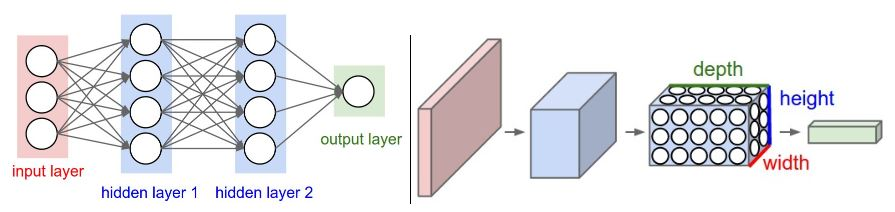
\includegraphics[width=15.8cm]{..//resources//images//conv_net.JPG} 
    \caption{Left: A regular 3-layer Neural Network. Right: A ConvNet arranges its neurons 
    in three dimensions (width, height, depth), as visualized in one of the layers. 
    Every layer of a ConvNet transforms the 3D input volume to a 3D output volume 
    of neuron activations. In this example, the red input layer holds the image, 
    so its width and height would be the dimensions of the image, 
    and the depth would be 3 (Red, Green, Blue channels) \cite{WEBSITE:cnn-for-visual-recognition}}
\end{figure}
\fi

În general, rețelele neuronale convoluționale, cunoscute și ca ConvNets, utilizează
3 tipuri de straturi pentru a construi arhitectura, și anume: convolutional layer, 
pooling layer și fully-connected layer. 

Un strat de convoluție \emph{(Convolutional Layer)}, este responsabil
de scanarea unei reprezentări sursă de tip imagine, aplicând un filtru de o anumită dimensiune,
cu scopul de a extrage caracteristici care pot fi importante pentru clasificare. Acest filtru 
mai este numit nucleu de convoluție \emph{(convolution kernel)}. Nucleul conține parametrii care
pot fi ajustați pentru a atinge cele mai precise predicții.

Spre exemplu, în cadrul unui nucleu de dimensiunea 5 x 5, pentru fiecare regiune de 5 x 5 pixeli, 
modelul calculează o serie de produse între valorea pixelului din imagine, la o anumită poziție
și parametrul corespunzător definit în filtru.

După încheierea convoluției, caracteristicile sunt comprimate \emph{(downsampled)}, urmând 
ca aceeași structură convoluțională să se repete. La început, convoluția identifică trăsături
din imaginea originală, apoi identifică sub-caracteristici în părți mai mici ale imaginii.
În cele din urmă, acest proces este
menit să identifice caracteristicile esențiale care pot ajuta la clasificarea imaginii.
Straturile de convoluție produc astfel unul sau mai multe imagini numite hărți de trăsături \emph{(feature maps)}, imagini 
care conțini caracteristici ce apațin imaginii originale, înainte de punerea în aplicare a 
nucleului de convoluție. Un exemplu de aplicare a două straturi convoluționale este 
prezentat în Figura 4.4.

\begin{figure}[h!]
    \centering
    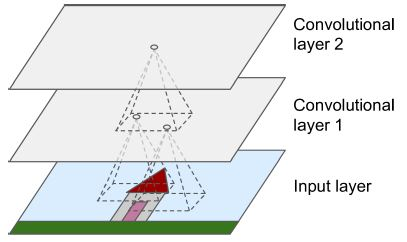
\includegraphics[width=9cm]{..//resources//images//conv_layer.JPG} 
    \caption{Două straturi de convoluție în cadrul unui CNN, aplicând câte un filtru pe o regiune 
    din imaginea de input \cite{Hands-On-Machine-Learning}.}
\end{figure}

Stratul de agregare, \emph{Pooling layer}, are rolul de a reduce/micșora dimensiunea 
imaginii de intrare, comprimând ieșirile unui strat convoluțional. Se consideră,
ca exemplu în Figura 4.5, un filtru de dimensiunea 2 x 2 care urmează a fi aplicat folosind agregarea asupra 
unei imagini de dimensiunea 4 x 4. Folosind acest filtru, există două strategii care pot fi 
aplicate:
\begin{enumerate}
    \item Calculul mediei valorilor din regiunea acoperită de filtru \emph{(mean pooling)}.
    \item Determinarea maximului din regiunea acoperită de filtru \emph{(max pooling)}.
\end{enumerate}

\begin{figure}[h!]
    \centering
    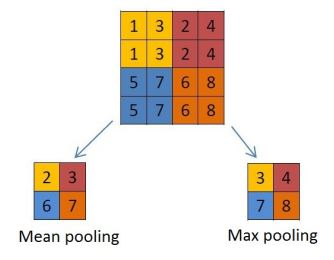
\includegraphics[width=9cm]{..//resources//images//pooling.JPG} 
    \caption{Operațiile de mean pooling (imaginea din stânga) și max pooling
    (imaginea din dreapta). 
    Elementele din straturile de pooling sunt obținute din matricea de intrare,
    din zona cu aceeași culoare. În acest caz, din matricea de intrare de dimensiunea 4 × 4
    se determină un rezultat cu dimensiunea 2 × 2 \cite{WEBSITE:rovislab}.}
\end{figure}

Straturile de convoluție și agregare sunt supuse unei funcții de activare cu rolul de a asigura
comportamentul neliniar al rețelei. Ca funcție de activare, de cele mai multe ori se folosește
ReLU \emph{(Rectified Linear Unit)}. Mai este cunoscută ca operația de rectificare.
ReLU este funcția de activare cel mai frecvent folosită în construirea 
modelelor de învățare profundă. Funcția returnează 0 dacă primește o intrare
negativă, iar pentru orice valoare pozitivă x, se returnează aceea valoare. 
Pe scurt, se definește ca:
\begin{equation*}
   f_{ReLU} (x) = max(0, x)
\end{equation*}

O componentă complet conectată, \emph{Fully connected}, are rolul de a realiza
clasificarea propriu zisă. Această componentă este o rețea neuronală clasică, la intrarea
căreia se furnizează feature map-urile, și la ieșirea căreia se aplică funcția de activare
\emph{softmax}. 

În matematică, funcția softmax, cunoscută și ca softargmax sau funcție exponențială 
normalizată, este o funcție care ia ca input un vector K de numere reale și îl normalizează 
într-o distribuție de probabilități, constând în probabilități K proporționale la valorile 
exponențiale ale numerelor din vectorul de intrare. Spre exemplu, înainte de 
aplicarea funcției softmax, unele componente vectoriale pot avea valori negative, sau mai mari
decât 1, fiind posibil ca suma tuturor componentelor să nu fie egală cu 1. Dar, 
aplicând softmax, fiecare componentă se va afla în intervalul $(0,1)$, ceea ce 
înseamnă că vor putea fi interpretate ca probabilități. Funcția softmax se definește
matematic astfel:

\begin{equation*}
    \sigma(z)_i = \frac{e^{z_i}}{\sum_{j=1}^{K}e^{z_j}}, i=1,...,K; z=(z_1,...,z_k)
 \end{equation*}
 

Astfel, ieșirea acestei componente este un vector de probabilități cu un număr de
componente egal cu numărul de clase. Fiecare componentă a vectorului reprezintă
probabilitatea ca imaginea dată ca input să se încadreze în clasa corespunzătoare.

Recapitulând întreg procesul, imaginea de la intrare conține o entitate care 
trebuie încadrată într-una din clasele preexistente. Input-ul este supus mai multor
operații de convoluție, agregare și rectificare, de fiecare dată generându-se
hărți de trăsături. Acestea conțin trăsături semnificative ale imaginii
inițiale. Trăsăturile sunt apoi supuse unui proces de clasificare prin intermediul
unei rețele neuronale complet conectate, rezultând o serie de
probabilități ca imaginea să aparțină fiecărei categorii. 

Arhitecturile tipice de CNN conțin câteva straturi convoluționale (fiecare având 
în continuarea lui câte un strat ReLU), apoi un strat de agregare, apoi alte câteva straturi
convoluționale, apoi un alt strat de agregare, și așa mai departe. Imaginea 
devine din ce în ce mai mică pe măsură ce progreseză prin rețea, devenind de asemenea 
din ce în ce mai profundă (adică, cu mai multe hărți de trăsături), datorită 
straturilor convoluționale. Schița unei arhitecturi convuluționale clasice este 
înfățișată în Figura 4.6.

\begin{figure}[h!]
    \centering
    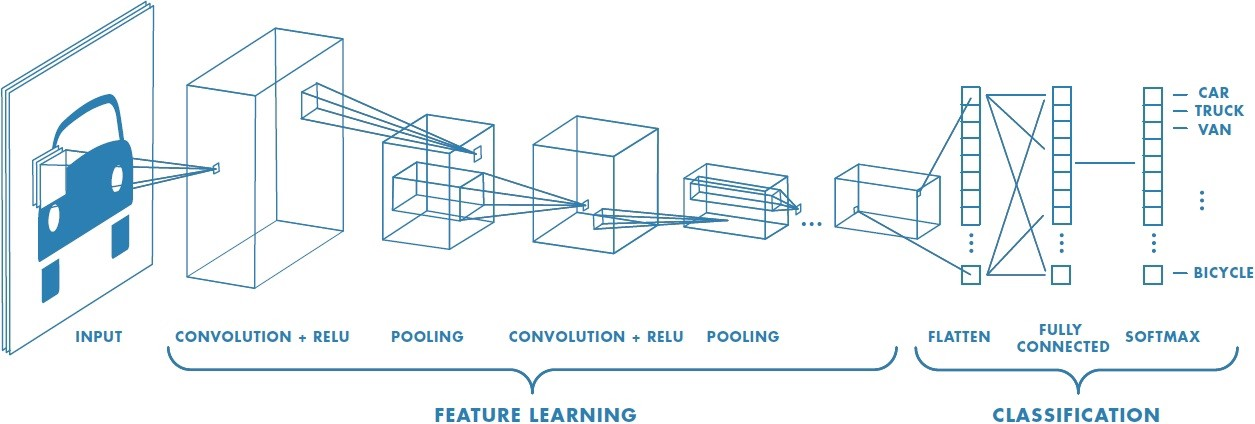
\includegraphics[width=15cm]{..//resources//images//conv_cnn.jpeg} 
    \caption{Arhitectură CNN. Se consideră o imagine ca input, care este supusă operațiilor corespunzătoare straturilor
    de convoluție și agregare. Rezultatul se propagă prin straturi complet conectate. 
    Ieșirea rețelei constă într-un vector de probabilități ce încadrează imaginea într-o mulțime
    de clase preexistente \cite{WEBSITE:medium-raghav}.}
\end{figure}

Există o multitudine de arhitecturi actuale folosite în mod uzual, unele 
fiind specializate pe rezolvarea anumitor probleme. Cu toate acestea, unele
sunt considerate de mare interes, fiind situate la baza acestui domeniu,
printre care:
\begin{itemize}
    \item LetNet-5: Este cea mai veche arhitectură convoluțională, fiind descrisă pentru prima oară 
    în 1998 cu scopul de a recunoaște cifre scrise de mână în cadrul documentelor, fiind concepută 
    pentru imagini cu rezoluție mică;
    \item AlexNet: Este o arhitectură 
    apărută după mai bine de un deceniu, în anul 2012, având 5 straturi convoluționale, acceptând 
    imagini de intrare considerabil mai mari în rezoluție, având nuclee de convoluție mai mari 
    în straturile inițiale (11 x 11). A fost antrenată cu ajutorul a două GPU-uri performante,
    fiind mai puternică decât arhitecturile precendete;
    \item VGG: Este arhitectura care a demonstrat creșterea performanței odată cu adâncimea mai 
    mare a rețelei, având un număr semnificativ de straturi de orice tip (16, 19), fiind printre 
    cele mai mari rețele utilizate în ceea ce privește numărul 
    de parametri care trebuie învățați.
\end{itemize}
\newpage
\subsection{Rețele de convingeri profunde}
Rețelele de convingeri profunde se prezintă ca o categorie de algoritmi care folosesc 
probabilitățile și învățarea nesupervizată pentru a produce rezultate. Sunt compuse 
din variabile latente(variabile care nu sunt observate direct, 
ci sunt mai degrabă deduse din alte variabile observate) binare, și conțin
atât straturi nedirecționate, cât și straturi direcționate.

Spre deosebire de alte modele, fiecare strat din cadrul unei rețete de convingeri profunde 
învață caracteristici folosind întreaga entitate de input. Prin comparație, CNN-urile 
utilizează primele straturi pentru a filtra entitatea de intrare, obținând doar 
caracteristicile de bază, straturile ulterioare recombinând 
informația din straturile inferioare. În cadrul rețelei, nodurile din fiecare strat sunt conectate la toate nodurile 
din stratul anterior si ulterior. Nodurile nu comunică lateral în cadrul aceluiași strat. 
De asemenea, nodurile din stratul ascuns îndeplinesc două roluri: acționează 
ca un strat ascuns față de nodurile care îl preced și ca straturi vizibile 
pentru nodurile care îl succed. Aceste noduri identifică corelații între date \cite{WEBSITE:conv2d-working-cnn}. 

Pentru antrenarea rețelelor de convingeri profunde,  
se folosesc algoritmi de tip greedy. Această abordare este specifică algoritmilor 
care implică luarea unei decizii la fiecare strat din secvență, găsind în cele 
din urmă un optim global. Învățarea se desfășoară de la un nivel la altul, 
ceea ce înseamnă că straturile rețelelor de convingeri profunde sunt instruite pe rând. 
Prin urmare, fiecare strat primește o versiune diferită a datelor și 
fiecare folosește ieșirea din stratul anterior ca intrare a acestora. 
Algoritmii de tip greedy sunt folosiți pentru a antrena rețele de convingeri profunde
deoarece sunt rapizi și eficienți \cite{WEBSITE:conv2d-working-cnn}. 
Mai mult, ajută la optimizarea parametriilor la fiecare strat.

În ceea ce privește ariile de aplicabilitate, acest tip de rețele pot fi utilizate 
cu succes în recunoașterea audio sau de imagini, dar și implementarea unor 
algoritmi de colectare a datelor în timp real (de exemplu, urmărirea mișcării
de obiecte sau de persoane). Recunoașterea de note sau acorduri dintr-o reprezentare audio 
are la bază clasificarea de imagini, în urma procesării sunetului și obținerea unei 
reprezentări pe baza trăsăturilor extrase. 

Rezultatele unei astfel de abordări 
vor fi prezentate în Capitolul 7, pe baza unei lucrări 
ștințifice care abordează diferite strategii, printre care și cea a rețelelor de 
convingeri profunde.

\chapter{Rezultate experimentale}
În acest capitol se va descrie soluția 
propusă, prin stabilirea setului de date, prezentarea 
arhitecturii rețelei neuronale și a etapelor intermediare construcției, și prin 
enunțarea rezultatelor finale obținute în urma antrenării și testării modelului.

\section{Descrierea soluție propuse}
Pentru construcția modelului de recunoaștere a acordurilor acustice, 
se va utiliza o rețea neuronală convoluțională. 
CNN-urile au crescut în popularitate în ultimii ani, mai ales în domeniul 
viziunii computerizate (\emph{computer vision}). 

În cadrul rețelelor neuronale convoluționale, imaginea construită sau aleasă
este folosită ca parametru de intrare pentru CNN, iar imaginea este trecută prin mai multe straturi, 
cum ar fi straturile convoluționale, straturile de agregare și starturile de activare.
Straturile convoluționale sunt construite din mai multe filtre, care pot fi interpretate individual,
fiecare învățând unele caracteristici superioare ale imaginii. 

În cadrul problemei de recunoaștere automată a acordurilor muzicale acustice,
detectarea acordurilor poate fi tratată în mod similar cu recunoașterea 
imaginilor, deoarece se pot crea imagini cu reprezentarea de tip chromagramă. Identificarea 
notelor sau a acordurile este mai simplă decât clasificarea imaginilor, întrucât nu implică 
învățarea anumitor texturi, rotiri sau scalări. 
Cu toate acestea, această problemă vine cu alte provocări. 
Notele muzicale din cadrul chromagramei nu sunt localizate într-o singură
regiune, în același mod în care sunt cele mai multe obiecte din imagini - o notă 
la o anumită frecvență fundamentală va fi compusă din armonice la multiplii acelei frecvențe.

În ciuda acestei provocări, CNN-urile au proprietăți avantajoase care pot fi aplicate 
cu succes în această problemă. Experimentele anterioare au sugerat că agregarea informațiilor
considerând mai multe cadre muzicale din același eșantion, determină obținerea unei predicții 
cu o performanță mai mare.
Astfel, convoluțiile aplicate asupra datelor de intrare permit modelului creat 
să învețe caracteristici muzicale polifonice valoroase.
\section{Setul de date}
Setul de date utilizat pentru antrenarea și evaluarea modelului convoluțional
creat este format din combinarea a 3 seturi de date pentru chitară,
disponibile online, asupra cărora s-au aplicat o serie de algoritmi de augmentare. 
Setul de date este astfel compus din:
\begin{itemize}
    \item 7398 de acorduri individuale, grupate în 16 fișiere audio de tip wav, aparținând 
Institutului de semantică muzicală Fraunhofer, din cadrul Universității tehnice Ilmenau, Germania. 
Setul de date se numește IDMT-SMT-CHORDS;
    \item 6580 de înregistrări audio, fiecare având în compoziție un singur acord, aparținând 
laboratorului de cercetări muzicale al Universității din New York, SUA, numit
GuitarSet\cite{Guitar-Set};
    \item 200 de fișiere audio pentru 10 tipuri de acorduri, fiind colectat de grupul 
de cercetare Motefiore al Universității din Liège, Belgia.
\end{itemize}

După aplicarea algoritmilor de augmentare asupra setului de date complet, s-a obținut 
un total de 58.577 de înregistrări audio de tip wav, grupate în cele 24+1 clase(24 de acorduri 
cu etichete corespunzătoare cunoscute, și o etichetă pentru orice alt acord care 
nu se încadrează).

Cele 24 de acorduri recunoscute de către sistem, împreună cu valorile numerice asociate sunt
următoarele(perechi de forma acord muzical-valoare asociată): 
A-0, A\#-1, A\#m-2, Am-3, B-4, Bm-5, C-6, C\#-7, C\#m-8, Cm-9, D-10, D\#-11, D\#m-12, Dm-13,
E-14, Em-15, F-16, F\#-17, F\#m-18, Fm-19, G-20, G\#-21, G\#m-22, Gm-23. Pentru orice alt acord 
care nu se încadrează în această înșiruire s-a creat perechea N-24 (acord necunoscut N, cu
valoarea asociată de 24). Distribuția datelor pe clase se poate observa în Figura 5.1.

\begin{figure}[h!]
    \centering
    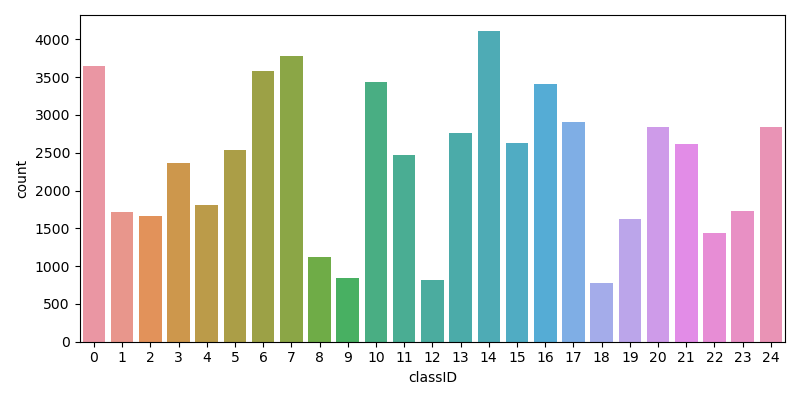
\includegraphics[width=14cm]{..//resources//images//myplot_new_distribution.png}
    \caption{Distribuția datelor pe clase, prin specificarea numărului de fișiere audio 
    disponibile pentru fiecare clasă asociată acordurilor muzicale.}
\end{figure}


\subsection{Augmentarea datelor}
Metodele de augmentare a datelor au rolul de a crește în mod artificial 
dimensiunea setului de date, generând multe variante realiste ale fiecărei 
instanțe set. Această procedură reduce posibilitatea de overfitting. 

Instanțele generate trebuie să fie cât mai realiste, astfel încât nimeni să nu fie 
capabil să diferențieze între varianta originală și cea augmentată (caz ideal, în realitate 
vor exista aspecte care le vor diferenția) \cite{Hands-On-Machine-Learning}.
Asupra acestui set de date s-au aplicat două metode de augmentare diferite, anume:
\begin{enumerate}
    \item Modicarea vitezei de redare, pentru fiecare instanță în parte, prin două metode:
    \begin{itemize}
        \item Incrementarea vitezei cu 1.25\% față de original;
        \item Decrementarea vitezei cu 0.75\% față de original;
        \item Decrementarea vitezei cu 0.55\% față de original (doar pentru un fragment 
        din setul de date inițial).
    \end{itemize}
    \item Injectarea unui zgomot de fundal, pentru fiecare fișier audio, prin adăugarea 
unei valori generate random în vectorul de date specific.
\end{enumerate}

\subsection{Normalizarea datelor}
Normalizarea este procesul de redimimensionare a datelor din intervalul 
inițial într-un alt interval prestabilit, cel mai frecvent în 
intervalul $[0,1]$. Algoritmul de normalizare folosit asupra 
setului de date este normalizarea $L-\infty$. 

Normalizarea $L-\infty$ este 
o strategie de normalizare prin care toate valorile unui vector de caracteristici sunt aduse 
în intervalul $[0,1]$, prin împărțirea fiecărei valori la maximul acelui vector \cite{Bonvini-Recognition}.
LibROSA oferă acest tip de normalizare ca fiind prestabilită pentru obținerea 
chromagramei, atât prin STFT, cât și prin transformata Q constantă. 
De asemenea, librăria oferă prestabilită valoarea pentru marginea inferioară 
acceptată, numită \emph{threshold}. Acest parametru are valoare 0, astfel 
orice valoarea sub 0 din vectorii caracteristici asociați chromagramei va fi ignorată
și setată cu valoarea 0.

\iffalse
Normalizarea datelor: utilizand algoritmul "L-inf normalization" - pagina 59 Bonvini;
Librosa oferă normalizarea de tip L-inf ca fiind prestabilită 
pentru obtinirea chromogramei atat cu STFT cat si cu Q-Constant.
De asemenea, prestabilita este si valorea pentru  threshold = 0.0, astfel orice frame 
din chromograma cu valorea sub 0 va fi ignorat si setat cu valorea 0 ("Pre-normalizare");
\fi

\newpage
\section{Extragerea trăsăturilor muzicale}
Extragerea trăsăturilor muzicale are la bază unul din algoritmii de 
procesare a semnalului sonor, mai precis, transformata Q constantă. 
Prezentarea teoretică și avantajele pe baza cărora a fost aleasă 
această metodă sunt prezentate în Capitolul 3. 

Pentru determinarea chromagramei utilizând metoda transformatei Q constante, 
s-au utilizat metodele de procesare oferite de către librăria LibROSA.
Astfel, metoda aferentă transformatei primește ca parametru fișierul 
audio de tip wav, o valoare pentru salt sau \emph{hop{\_}length} egală
cu 512 și valoarea opțională pentru numărul de semitonuri distincte 
la nivelul unui octave muzicale, valoare egală cu 24. 

Durata acceptată la încărcarea unui fișier audio (care reprezintă 
înregistrarea unui acord muzical) este de 2 secunde. Astfel, 
cunoscând parametrii aplicați tranformatei și durata admisă pentru
un fișier audio, chromagrama construită are o dimensiune standard 
de 24x87, adică fiecare din cei 24 de vectori caracteristici are 
87 de valori de tip double în intervalul $[0,1]$.
În cazul în care înregistrarea are mai puțin de două secunde, se adaugă valori de 0 
la vectorii caracteristici, 
până se ajunge la dimensiunea standard.

Pentru a eficientiza procesarea fiecărui fișier audio prin 
aplicarea tranformatei Q constantă, acestea vor fi procesate 
în paralel, prin crearea a 10 threaduri, care să execute 
aceeași sarcină pe intervale diferite din setul de date audio.
Astfel, clasa care definește sarcinile unui thread se inițializează 
astfel: 
\begin{python}
    import threading
    import librosa

    processed_data = []
    class ChromaProcessingThread(threading.Thread):
        def __init__(self, threadID, name, start_point, stop, data_labeled):
            threading.Thread.__init__(self)
            self.threadID = threadID
            self.name = name
            self.start_point = start_point
            self.stop = stop
            self.data_labeled = data_labeled
\end{python}

Campul \emph{data{\_}labeled} este un obiect construit pe baza datelor 
și a unui fișier Excel preprocesat, care conține informații cu 
privire la o înregistrare audio. Aceste informații sunt: calea absolută 
către acel fișier audio de tip wav, eticheta de ieșire corespunzătoare 
acelui fișier (numele acordului muzical) și valorea numerică 
asociată etichetei (cuprinsă între 0 și 24).

După inițializarea celor 10 threaduri, acestea sunt pornite, iar 
rularea paralelă de procesare a sunetelor și obținerea reprezentărilor 
prin chromagramă începe. Fiecare thread este așteptat cu o parcurgere 
finală, prin intermediul unor join-uri. Astfel, metoda \emph{run}, implementată 
de clasa ChromaProcessingThread, se definește în felul următor:

\begin{python}
    def run(self):
        print("Starting " + self.__name + "/n")

        for i in range(self.__start_point, self.__stop):
            song, sr = librosa.load(self.__data_labeled.loc[i].file_name, duration=2)

            # Compute chromagram
            chromagram = librosa.feature.chroma_cqt(song, 
                                sr=sr, 
                                hop_length=AUDIO_CONSTANTS.hop_length, 
                                n_chroma=24,
                                n_octaves=7)

            # Reshape chroma matrix (if it is necessary)
            aux_chroma = []
            if chromagram.shape != (24, 87):
                for row in chromagram:
                    while len(row) < 87:
                        row = np.append(row, [0])

                    aux_chroma.append(row)    
                chromagram = np.array(aux_chroma)

            # Save processed chroma matrix
            processed_data.append((chromagram, self.__data_labeled.loc[i].classID))

        # Thread @self.__name is done
        print("Exiting /n" + self.__name + "/n")
\end{python}

După finalizarea procesării din partea celor 10 threaduri, vectorul \emph{processed{\_}data}
ce conține toate chromagramele sub formă de matrici pentru 
toate fișierele audio va fi salvat într-un fișier local de 
tip numpy. Din acest fișier vor fi incărcate datele în etapa următoare 
pentru antrenarea și testarea rețelei neuronale convoluționale. Salvarea 
în fișierul numpy corespunzătoar se face prin următoarea secțiune de cod.
\begin{python}
    import numpy as np

    np.save(AUDIO_CONSTANTS.RESOURCES_PATH +
            "//data_chroma24_hop512.npy", processed_data)

\end{python}

\iffalse
\begin{python}
    song, sr = librosa.load(self.data_labeled.loc[i].file_name, duration=2)
    chromagram = librosa.feature.chroma_cqt(song, sr=sr, 
                            hop_length=AUDIO_CONSTANTS.hop_length, 
                            n_chroma=24,
                            n_octaves=7)
\end{python}
\fi

\newpage
\section{Detectarea tranzițiilor muzicale}
Detectarea tranzițiilor muzicale, numită și \emph{onset detection}, este 
cunoscută ca o sarcină de găsire a punctelor/vârfurilor de pornire \emph{(peaks)},
ale tututor evenimentelor muzicale din cadrul unui semnal audio.
Problema detecției este una complexă, care poate avea la rândul 
ei mai multe abordări, în mod simiar cu procesarea sunetului \cite{WEBSITE:onset-detection}. 

Sistemul de recunoaștere automată a acordurilor muzicale 
este construit și antrenat pentru acorduri și înregistrări 
individuale. Pentru a putea aplica sistemul asupra pieselor 
sau înregistrărilor complexe, care conțin o serie de acorduri 
diferite, ce se schimbă frecvent, este nevoie de a detecta cu 
exactitate care este momentul în care se realizează trecerea 
de la un acord la altul \emph{(localization)}. Dacă se 
descoperă acele puncte pe axa timpului, se poate aplica 
algoritmul de recunoaștere pe toate intervalele determinate 
de punctele consecutive.

LibROSA oferă o metodă clasică de detectare a tranzițiilor, bazată 
pe lucrarea lui Bock, Krebs și Schedl \cite{Evaluating-the-online-capabilities-of-Onset-detection-methods}. Metoda este compusă 
din 3 pași:
\begin{itemize}
    \item Se compune o funcție ce denotă modificări locale ale proprietăților 
semnalului, cum ar fi energia. Este cunoscută ca funcția de noutate spectrală sau 
\emph{novelty function};
    \item Se găsesc vârfurile în funcția de noutate spectrală;
    \item Se aplică backtracking de la fiecare vârf la un minim local precendent, pentru 
a găsi punctele de segmentare, astfel încât tranziția să apară la scurt timp după 
începutul segmentului \cite{WEBSITE:onset-detection}. Figura 5.2 prezintă care sunt 
vârfurile evenimentelor muzicale descoperite prin aplicarea algoritmului de detecție unei înregistări audio.
\end{itemize}

\begin{figure}[h!]
    \centering
    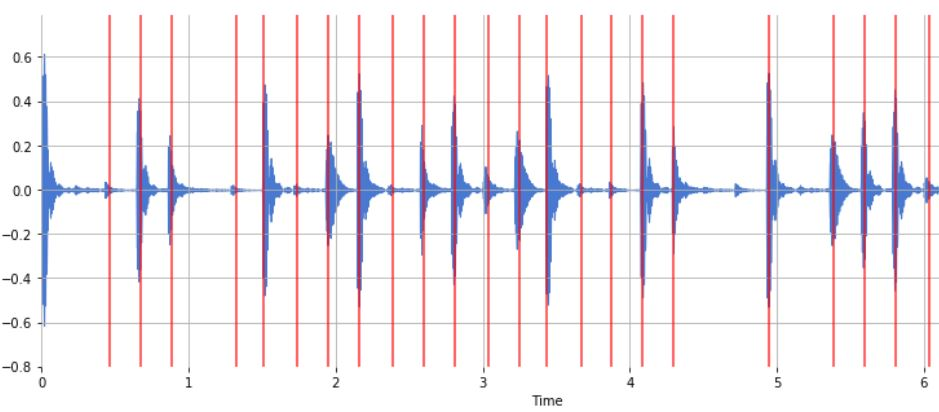
\includegraphics[width=15cm]{..//resources//images//wave_onset_detection.JPG} 
    \caption{Tranzițiile muzicale detectate (reprezentate prin linii roșii) 
pentru o înregistrare de aproximativ 6 secunde (reprezentată sub forma unei unde sonore albastre) \cite{WEBSITE:onset-detection}.}
\end{figure}

Întrucât segmentele determinate de tranzițiile între evenimentele muzicale 
descoperite în urma aplicării algoritmului sunt exacte și marchează foarte clar 
care sunt intervalele de timp cu evenimente muzicale diferite (acorduri muzicale), 
se aplică acest algoritm asupra pieselor sau înregistrărilor muzicale acustice, 
cu durata mai mare de două secunde. Astfel, aplicarea metodei de detectare 
a tranzițiilor se realizează în felul următor:

\begin{python}
    # Consider a complex audio recording
    audio_file = "//Let it Be Strum Guitar Cover.wav"
    # Load audio file
    song, sr = librosa.load(audio_file)
    # Compute the frame indices for estimated onsets in a signal
    onset_frames = librosa.onset.onset_detect(song, sr=sr, 
                                              backtrack=True)  
    # Convert onsets to units of seconds
    onset_times = librosa.frames_to_time(onset_frames)                                    
\end{python}

Vectorul \emph{onset\_times} conține unități de timp din intervalul de desfășurare 
a piesei audio, asupra căreia s-a aplicat metoda de detectarea a tranzițiilor.
Pentru a recunoaște care sunt acordurile acestei piese, se vor evalua, 
prin intermediul modelului neuronal, toate intervalele de timp consecutive, pe 
baza unităților de timp determinate. 

În urma aplicării acestei strategii, s-au 
observat două situații de excepție. În primul rând, dacă unul din intervalele 
determinate este prea scurt, modelul neuronal nu oferă predicții corecte 
(deoarece pe acel interval scurt, nu se extrag caracteristici suficiente), ceea ce 
a determinat adăugarea unei constante \emph{beta} care să marcheze valoarea minimă 
pentru ca un interval să fie considerat valid pentru predicție. Astfel, dacă un interval 
este prea scurt, se va încerca concatenarea cu următorul interval, până când se va construi 
un interval valid. În al doilea rând, este posibil ca un interval să fie prea lung. 
Această situație este mai simplă, intervalul fiind supus divizării. Cu aceste restricții
stabilite, procesarea și predicția intervalelor determinate de tranzițiile 
detectate se realizează astfel:

\begin{python}
beta = 0.75; i = 0
while i < (len(onset_times) - 1):
    offsetValue = onset_times[i]
    diff = onset_times[i + 1] - offsetValue
    while diff < beta and i < (len(onset_times) - 1) 
        and i < (len(onset_times) - 1):
            diff = onset_times[i + 1] - offsetValue
            i = i + 1
    if diff > 2:
        x = diff - 2
        diff = diff - x
    # Load the interval from original audio file
    song, sr = librosa.load(audio_file,
                            offset=offsetValue, 
                            duration=diff)
    # Compute chromagram(Extragerea trasaturilor muzicale)
    prediction = model.predict_classes(np.array([chromagram]))
\end{python}

\iffalse
\begin{figure}[h!]
    \centering
    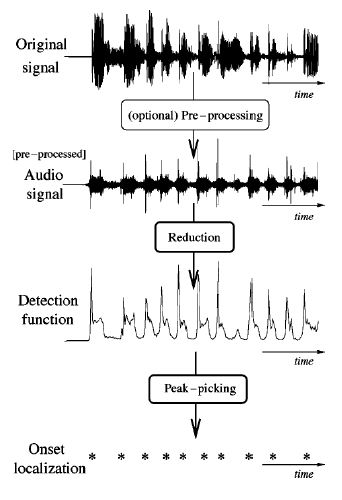
\includegraphics[width=10cm]{..//resources//images//onset_detection.JPG} 
    \caption{}
\end{figure}
\fi

\newpage
\section{Construirea, antrenarea și evaluarea modelului neuronal convoluțional}

Pentru construirea modelului convoluțional s-a folosit o secvență de
straturi specializate, așezate într-o ordine bine definită pentru 
a spori capacitatea de învățare. Straturile utilizate sunt:
\begin{itemize}
    \item Sequencial: Cel mai simplu model este definit folosind clasa Sequencial. Clasa definește 
o stivă liniară de straturi;
    \item ConvBlock: Definește un strat de convoluție 2D. Un strat de convoluție 2D înseamnă că 
    input-ul operației de convoluție este tridimensional (3D). Cu toate acestea, acest strat este considerat a fi de tip "2D" 
    deoarece mișcarea filtrului peste chromagramă
    se întâmplă în două dimensiuni. Filtrul este aplicat pe chromagramă de trei ori, 
    o dată pentru fiecare din cele trei straturi \cite{WEBSITE:conv2d-working-cnn};
    \item BatchNormalization: Normalizarea lotului sau \emph{batch normalization},
este o tehnică de normalizare a activării nodurilor din straturile intermediare 
ale unei rețele neuronale profunde. Tendința sa de a îmbunătăți precizia și de a 
accelera antrenamentul, au determinat ca această tehnică să fie preferată și
integrată în numeroase rețele de învățare profundă \cite{Understanding-Batch-Normalization}.
    \item MaxPooling: Reprezintă un strat clasic de agregare prin metoda 
determinării maximului din regiunea acoperită de filtru; 
    \item Dropout: Abandonarea, cunoscută drept \emph{dropout}, este o metodă de regularizare 
a rețelelor neuronale. Este o tehnică prin care anumiți neuroni selectați în mod aleator sunt ignorați
în timpul antrenamentului \cite{Hands-On-Machine-Learning}. Astfel, contribuția acestor neuroni la activarea altor neuroni este
îndepărtată temporar și orice actualizarea a parametrilor în rețea nu se va aplica pentru
acești neuroni. \\
Efectul este că rețeaua devine mai puțin sensibilă la parametrii specifici, rezultând o rețea 
capabililă să generalizeze mai bine orice fel de input și este mai puțin probabil ca rețeaua 
să se specializeze doar pentru un anumit set de date \emph{(avoiding overfitting)};
    \item Dense: Este un strat clasic de rețea neuronală complet conectată.
    Fiecare nod de intrare este conectat la fiecare nod de ieșire.
\end{itemize}

Astfel, cunoscând rolul fiecărui strat în parte, împreună cu funcțiile de activare
ReLU și Softmax, arhitectura 
rețelei convoluționale construite este prezentată în Figura 5.3.
\begin{figure}[h!]
    \centering
    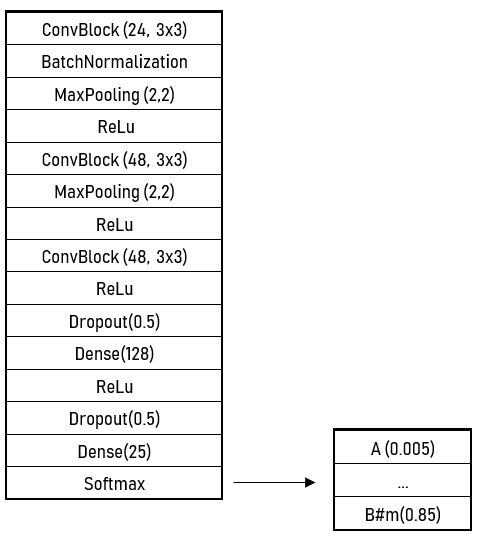
\includegraphics[width=10cm]{..//resources//cnn_arhitecture_image.JPG} 
    \caption{Arhitectura rețelei convoluționale construite. Numărul filtrelor 
    și dimensiunea nucleului de convoluție sunt indicate între paranteze, pentru 
    fiecare ConvBlock. Funcția de activare softmax este folosită în ultimul 
    strat dens.}
\end{figure}

Pentru a observa starea rulării programului, dar și pentru a 
ține o arhivă a etapelor parcurse, în cadrul proiectul s-a integrat
un sistem de logare \emph{(logging)}, care scrie într-un fișier 
de logare (jurnal) diferite mesaje, având un format prestabilit. Instanțierea sistemului de logare 
s-a realizat prin metoda: 
\begin{python}
    import logging
    import logging.config
    import yaml

    def logging_setup():
        with open(LOGGING_FILE_PATH, 'r') as f:
            config = yaml.safe_load(f.read())
            # Config logging using a dictionary
            logging.config.dictConfig(config)
\end{python}
Spre exemplu, o linie din jurnal arată astfel:

$2020-04-07 14:52:37,717 - src.modelling.cnntrain - INFO - Start Training Process$

Cu setul de date procesat în urma 
extragerii trăsăturilor muzicale pentru fiecare fișier audio 
și modelul convoluțional construit, mai rămân de stabilit 
valorile unor parametrii înainte de startul procesului de învățare. 

În primul rând, pentru antrenare, respectiv testare, setul de date va fi distribuit 
în mod aleator astfel: 80\% din 
numărul total de instanțe vor fi utilizate pentru antrenare, în timp 
ce restul de 20\% vor fi folosite pentru testarea modelului convoluțional.

\newpage
Setul de date procesat a fost încărcat în memorie din fișierul 
numpy corespunzător, astfel:
\begin{python}
    import numpy as np
    from science.utils import constants as AUDIO_CONSTANTS

    # Load computed dataset from .npy file
    dataset = np.load(AUDIO_CONSTANTS.RESOURCES_PATH 
                      + "//models//data_chroma24_hop512_beta_V3.npy", 
                      allow_pickle=True)
\end{python}

Pentru determinarea erorii sau a valorii pentru \emph{loss}, s-a folosit o strategie 
bazată pe entropie încrucișată. 
Entropia încrucișată 
compară predicția modelului cu valoarea etichetei corespunzătoare. 
Valoarea ei scade, pe măsură ce predicția devine din ce în ce mai precisă. 
Ea devine zero dacă predicția este perfectă \cite{Hands-On-Machine-Learning}.
Astfel, entropia încrucișată este o funcție de pierdere pentru a 
forma un model de clasificare.

Numărul de epoci setat este de 25. Această valoare determină de 
câte ori sistemul va repeta procesul de antrenare asupra datelor
corespunzătoare, acesta învățând de la o etapă la alta, devenind tot mai precis, 
cu o eroare din ce în ce mai mică.

În ceea ce privește algoritmul de optimizare, s-a 
ales algoritmul de optimizare Adam, cu dimensiunea unui bloc de 64 \emph{(batch{\_}size)}.
Adam este o metodă de adaptare a ratei de învățare, ceea ce înseamnă că rata de învățare
este calculată individual pentru diferiți parametri \cite{Hands-On-Machine-Learning}.

Întrucât librăria folosită pentru construirea modelului este Keras, 
se acceptă setarea ca parametru a unei instanțe pentru 
vizualizarea unor rezultate intermediare în timpul antrenării. Instanța este 
un obiect de tip TensorBoard, și se aplică modelului prin parametrul \emph{callbacks}.
De asemenea, tot ca parametru se poate seta o instanță pentru 
monitorizarea rezultatelor. Astfel, asupra modelului s-a aplicat o instanță de tip \emph{EarlyStopping} 
care are rolul de a opri antrenamentul în momentul în care una din
valorile monitorizate a încetat să se îmbunătățească. 

Cu toate aceste valori cunoscute, înțelese și setate corespunzător pentru rețeaua 
neuronală convoluțională, antrenarea poate începe cu succes. Metoda de antrenare 
utilizată în proiect este afișată în următoarea secțiune de cod.

\begin{python}
    import keras
    import logging
    import os

    def train(self, X_train, Y_train, X_test, Y_test):
        logger.info("Start training cnn model")

        # Compile model
        self.model.compile(
            optimizer="Adam",
            loss="categorical_crossentropy",
            metrics=['accuracy', precision, recall, f1measure])

        # TensorBoard Logging
        log_dir = os.path.join(AUDIO_CONSTANTS.LOGGING_PATH, datetime.datetime.now().strftime("%Y%m%d-%H%M%S"))
        tensorboard_callback = keras.callbacks.TensorBoard(log_dir=log_dir, histogram_freq=1)
        logger.info("Tensorboard Logging Started")
        
        # Start training
        self.__history = self.__model.fit(
            x=X_train,
            y=Y_train,
            epochs=25,
            batch_size=64,
            validation_data=(X_test, Y_test),
            callbacks=[tensorboard_callback,
                       EarlyStopping(monitor='val_loss', 
                       verbose=1, patience=2)])
        logger.info("Training completed")
\end{python}

După finalizarea antrenării, s-a realizat evaluarea modelului neuronal convoluțional 
pentru a calcula valorile metricilor la antrenare, dar cel mai important la testare, 
asupra unor date noi, care nu au mai fost "văzute" de către sistem. 
Valorile lor au fost salvate prin sistemul de logare al proiectului, urmând 
a fi preluate din jurnal pentru concluzii. Secțiunea de cod 
care realizează evaluarea este următoarea:

\begin{python}
    def evaluate(self, X_train, Y_train, X_test, Y_test):
        self.score_train = self.model.evaluate(
            x=X_train,
            y=Y_train)

        self.score_test = self.model.evaluate(
            x=X_test,
            y=Y_test)

        logger.info(f'Train loss: {self.score_train[0]}')
        logger.info(f'Train accuracy: {self.score_train[1]}')
        logger.info(f'Train precision: {self.score_train[2]}')
        logger.info(f'Train recall: {self.score_train[3]}')
        logger.info(f'Train f1-score: {self.score_train[4]}')

        logger.info(f'Test loss: {self.score_test[0]}')
        logger.info(f'Test accuracy: {self.score_test[1]}')
        logger.info(f'Test precision: {self.score_test[2]}')
        logger.info(f'Test recall: {self.score_test[3]}')
        logger.info(f'Test f1-score: {self.score_test[4]}')
\end{python}


\iffalse
\section{Parametrii experimentali}
\fi

\newpage
\section{Rezultate}
Pentru evaluarea performanței modelului convoluțional 
se vor introduce și utiliza câteva metrici de calcul.
Funcțiile asociate unor metrici de calcul sunt similare 
cu funcțiile pentru gestionarea erorii (loss-ului), 
cu excepția faptului că rezultatele evaluării unei metrici 
nu sunt utilizate la antrenarea modelului.
Metricile utilizate au fost acuratețe, precizie, recall și scorul F. 
Pentru a defini mai clar modul de calcul al acestor măsurători, se vor 
introduce următoarele variabile:
\begin{itemize}
    \item True Positives (TP): Numărul de cazuri cu predicția DA, 
    și valoarea reală DA;
    \item True Negatives (TN): Numărul de cazuri cu predicția NU, 
    și valoarea reală NU;
    \item False Positives (FP): Numărul de cazuri cu predicția DA, 
    și valoarea reală NU;
    \item False Negatives (FN): Numărul de cazuri cu predicția NU, 
    și valoarea reală DA.
\end{itemize}

\iffalse
True Positives (TP): Numărul de cazuri în care predicția este DA, 
iar valoarea reală este DA. \\
True Negatives (TN): Numărul de cazuri în care predicția este NU, 
iar valoarea reală este NU. \\
False Positives (FP): Numărul de cazuri în care predicția este DA, 
iar valoarea reală este NU. \\
False Negatives (FN): Numărul de cazuri în care predicția este NU, 
iar valoarea reală este DA.
\fi

Metricile alese au valori relevante doar în cazul în care există un  
număr echilibrat de probe pentru fiecare clasă în parte. 
De exemplu, se consideră existența a 98\% probe din clasa A și 2\% 
eșantioane din clasa B în setul de antrenament. Modelul obținut 
poate obține cu ușurință acuratețea de 98\% prezicând corect fiecare 
probă aparținând clasei A. Valoarea nu este însă una reală, modelul 
nefiind pregătit să recunoască instanțe ale clasei B. 

În cazul setului de date utilizat această problemă nu există, 
fișierele audio fiind distribuite în mod echilibrat în cele 25 de clase.
Cunoscând măsurătorile auxiliare și proprietatea 
de echilibru în distribuția datelor, metricile utilizate pot fi 
folosite cu succes. Acestea se definesc 
prin formulele următoare:

\begin{equation*}
    Acuratete (A) = \frac{TP+TN}{TP+TN+FP+FN} 
\end{equation*}

\begin{equation*}
    Recall (R) = \frac{TP}{TP+FN} 
\end{equation*}

\begin{equation*}
    Precizie (P) = \frac{TP}{TP+FP} 
\end{equation*}

\begin{equation*}
    Scor-F = \frac{2 \cdot R \cdot P}{R + P} 
\end{equation*}

Aceste metrici au fost aplicate la compilarea modelului neuronal
convoluțional. Rezultatele obținute sunt prezentate în Tabelul 5.1.

\begin{table}[h!]
    \begin{center}
        \begin{tabular}{ | c | c | c | c | c | }
            \hline 
                Etapă & Acuratețe & Precizie & Recall & Scor-F \\
                \hline \hline 
                Antrenare & 97.23\% & 98.38\% & 95.85\% & 97.05\%  \\
                \hline
                Testare & 89.75\% & 93.66\% & 86.67\% & 89.98\%  \\
            \hline
        \end{tabular}
        \caption{Rezultate obținute, în urma celor două etape: antrenare și testare.}
    \end{center}
\end{table}

Observarea și interpretarea rezultatelor scot în evidență eficiența 
și buna construire a unei rețele neuronale convoluționale, în 
contextul recunoașterii automate a partiturilor muzicale, cu
focus pe acordurile muzicale acustice. Toate metricile 
de calcul au valori de peste 89\%, fiind evitat cu succes overfitting-ul.
Precizia ridicată în recunoașterea și diferențirea acordurilor 
este datorată unei arhitecturi convoluționale corecte, cu straturi 
așezate în mod corespunzător, rețeaua având o adâncime suficientă.
Rezultatele bune se datorează și utilizării unei reprezentări 
potrivite, chromagrama fiind compusă din informații polifonice 
muzicale valoroare, care au ajutat modelul să învețe cu succes
cele mai importante trăsături, la fiecare pas.

Pentru a observa evoluția proceselor de antrenare și testare, și impactul 
întregului proces asupra metricilor de calcul, s-au realizat două grafice 
pentru a evidenția scăderea loss-ului și creșterea acurateții.
Astfel, Figura 5.4 prezintă valorile pe care le-a avut eroarea(loss-ul), dar 
și acuratețea, 
pe parcursul celor 25 de epoci. Se observă o scădere relativ exponențială,
valorile loss-ului la antrenare, respectiv la testare fiind apropiate.
În ceea ce privește valorile pentru acuratețe, este evidențiat un trend 
ascendent, valorile pentru antrenare și testare 
fiind apropiate spre ultimele epoci (sugerând o învățare 
corectă și echilibrată).

\begin{figure}[h!]
    \centering
    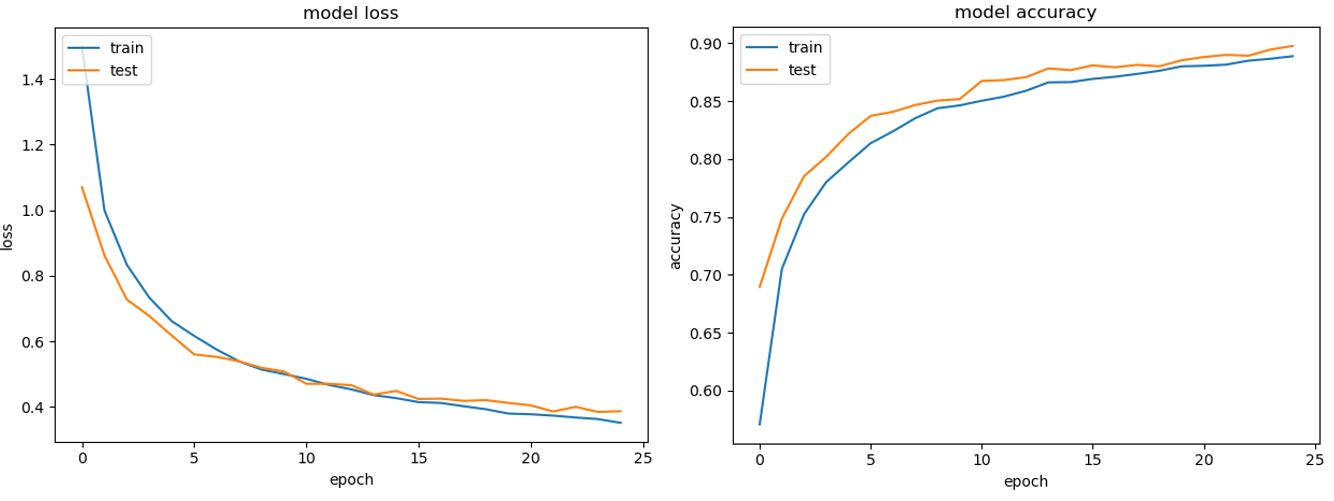
\includegraphics[width=15.8cm]{..//resources//images//loss_accuracy.JPG} 
    \caption{Evoluția valorilor pentru loss (stânga) și acuratețe (dreapta), 
    la antrenare și testare. Cele două grafice au fost realizate la finalul procesului 
    de învățare, folosind matplotlib.pyplot.}
\end{figure}

\iffalse
\begin{figure}[h!]
    \centering
    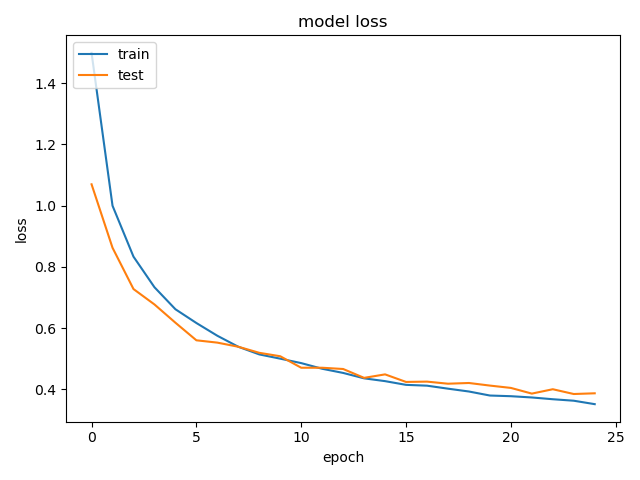
\includegraphics[width=10.6cm]{..//resources//images//model_loss.png} 
    \caption{Evoluția valorii pentru loss, la antrenare și testare.}
\end{figure}

\begin{figure}[h!]
    \centering
    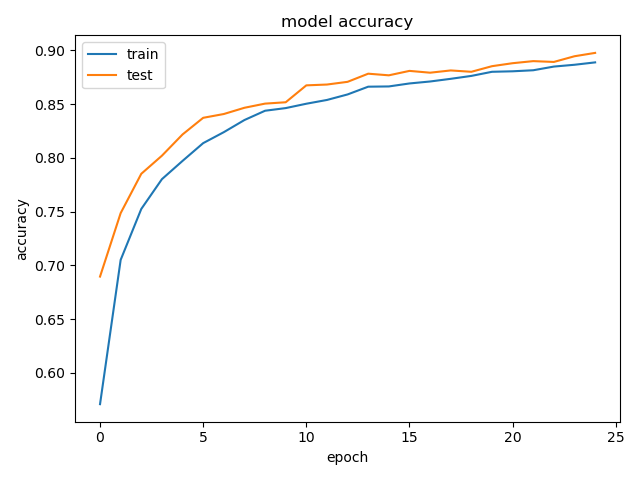
\includegraphics[width=10.6cm]{..//resources//images//model_accuracy.png} 
    \caption{Evoluția valorii pentru acuratețe, la antrenare și testare.}
\end{figure}
\fi


\subsection{Validare încrucișată}
Rezultatele prezentate în secțiunea anterioară sunt obținute prin 
amestecarea setului de date, și extragerea, în mod aleator, a celor 
două grupuri pentru a realiza antrenarea, respectiv testarea modelului 
neuronal convoluțional. În acest mod, validarea modelului este una simplă,
prin aplicarea celor două seturi disjuncte. 

Cu toate acestea, există metode care pot estima/valida mult mai bine 
performanța modelului, prin realizarea unei analize statistice 
asupra acestuia, în raport cu setul de date existent. 
Una din metode se numește validare încrucișată 
\emph{(cross-validation)}.

Validarea încrucișată este o procedură de eșantionare 
folosită pentru a evalua modele de învățare automată, 
în momentul în care setul de date este limitat \cite{WEBSITE:k-fold-cross-validation}.
Procedura are un singur parametru esențial, notat cu k, iar 
acesta se referă la numărul de grupuri în care un set 
de date trebuie împărțit. Ca atare, metoda este cunoscută
și ca \emph{k-fold cross-validation}.

Procedura este utilizată în principal pentru algoritmii 
de învățare automată, cu scopul de a estima abilitatea 
unui model de a generaliza caracteristicile învățate 
asupra datelor nevăzute. 
Metoda este una populară, deoarece
este simplă de înțeles, și are ca rezultat o estimare 
mai puțin optimistă, dar mai aproape de realitate, prin comparație 
cu metoda validării simple, care realizează o singură divizare 
pentru antrenare și testare \cite{WEBSITE:k-fold-cross-validation}.

Validarea încrucișată urmează o serie de pași:
\begin{itemize}
    \setlength\itemsep{0.2em}
    \item Setul de date este modificat în mod aleator, și împărțit în k grupuri;
    \item Pentru fiecare grup, se aplică următorii pași:
    \begin{itemize}
        \item Se consideră grupul ca set pentru testare, în timp ce 
    grupurile rămase sunt unite pentru setul de antrenament;
        \item Se construiește un model pe baza setului de antrenament, 
    și se evaluează folosind setul de testare (grupul curent);
        \item Se păstrează scorurile, în timp ce modelul este aruncat (fiindcă nu va fi folosit, 
        având un scop doar pentru evaluare) \cite{WEBSITE:k-fold-cross-validation}.
    \end{itemize}
    \item Se adună toate rezultatale obținute și se realizează o medie a 
    acestora.
\end{itemize}

Este important de precizat faptul că fiecare informație din setul 
de date care este atribuită unui grup individual rămâne 
în acel grup pe toată durata procedurii. În acest fel, fiecare 
grup are șansa de a fi utilizat o singură dată pentru testare, și de $k-1$ 
ori pentru antrenare, obținându-se astfel o evaluare 
încrucișată a modelului neuronal creat \cite{WEBSITE:k-fold-cross-validation}. 
Această metodă 
a fost aplicată asupra modelului convoluțional existent și 
a setului de date muzical existent. Valorea aleasă pentru k a 
fost 5, iar rezultatele obținute prin realizarea 
unei medii a celor k rezultate intermediare 
pot fi observate în Tabelul 5.2.

\begin{table}[h!]
    \begin{center}
        \begin{tabular}{ | c | c | c | c | c | }
            \hline 
                Etapă & Acuratețe & Precizie & Recall & Scor-F \\
                \hline \hline 
                Antrenare & 96.11\% & 98.03\% & 93.42\% & 95.61\%  \\
                \hline
                Testare & 91.61\% & 95.43\% & 88.25\% & 91.64\%  \\
            \hline
        \end{tabular}
        \caption{Rezultatele determinate prin aplicarea validării încrucișate.}
    \end{center}
\end{table}

Se observă că aceste rezultate sunt apropiate de cele obținute prin validare simplă.
Acest fapt confirmă concluziile inițiale cu privirea la modelul existent, acesta fiind 
unul adecvant pentru problema recunoașterii automate a acordurilor muzicale. 


\chapter{Aplicația sistemului}
Acest capitol urmărește prezentarea proiectului din 
perspectiva ingineriei de sistem, prin analiza 
limbajele de programare și a mediile de dezvoltare folosite, 
dar cel mai important, prezentând arhitectura sistemului,
prin evidențierea modelelor software, atât la nivel teoretic, 
cât și practic, prin construirea diagramelor specifice.
\section{Mediu de lucru}
\subsection{Back-end}
\iffalse
Limbaj: Python; Env: Google Colab, Visual Studio Code, PyCharm
\fi
Limbajul de programare folosit pentru realizarea proiectului de back-end este Python.
Este un limbaj de de nivel înalt, orientat obiect, ce 
pune accent pe expresivitatea și înțelegerea ușoară a codului.
Constucția sa la nivel înalt, în combinație cu tastarea dinamică și
legarea dinamică, îl fac foarte atractiv pentru dezvoltarea rapidă a aplicațiilor,
precum și pentru utilizarea în scripting sau ca limbaj de legătură pentru 
a conecta componentele existente împreună \cite{WEBSITE:python}.

Python se caracterizează prin lizibilitate și, prin urmare, reduce costurile 
de întreținere a unui program. Este construit să suporte module și pachete, 
care încurajează modularitatea programului și reutilizarea codului. 
Interpretorul Python și biblioteca extinsă standard sunt disponibile 
în formă sursă sau în formă binară, fără taxe, pentru toate platformele 
majore, fiind posibilă distribuirea în mod liber \cite{WEBSITE:python}.

Python este unul din limbajele favorite în rândul dezvoltatorilor, fiind 
potrivit pentru multe tipuri de aplicații. În mod particular însă, 
este considerat ca fiind cea mai bună alegere pentru proiectele care implică 
inteligența artificială. Acest lucru este datorat faptului că limbajul 
conține foarte multe biblioteci și framework-uri externe, care facilitează 
procesul de codare și economisește timpul de dezvoltare. Învățarea automată 
și învățarea profundă sunt foarte bine tratate, prin numeroase librării,
printre acestea se numără NumPy, folosit pentru calcul științific, 
SciPy pentru calcule avansate și 
scikit-learning pentru minerirea datelor și analiza datelor, 
fiind printre cele mai populare biblioteci, 
lucrând alături de framework-uri externe puternice precum TensorFlow, 
Keras, CNTK sau Apache Spark.

Atât învățarea automată cat și cea profundă se bazează pe 
algoritmi extrem de complecși și pe fluxuri de lucru
în mai multe etape. Prin urmare, cu cât un dezvoltator 
trebuie să se îngrijoreze mai puțin de complexitatea 
codificării, cu atât mai mult se poate concentra pe găsirea unei soluții
optime și atingerea obiectivelor proiectului. 
Sintaxa simplă în Python determină o dezvoltare mai rapidă 
decât alte limbaje de programare și permite dezvoltatorului să 
testeze rapid algoritmii fără a fi nevoie să îi implementeze.

În ceea ce privește mediul de dezvoltare (IDE), au fost utilizate 
două medii diferite, în funcție de complexitatea proiectului. 
În primă fază, pentru realizarea 
unui prototip de model neuronal și acumularea de deprinderi utilizând 
librării ca TensorFlow, Keras, NumPy sau LibROSA, s-a utilizat
Google Colab. Acesta este un mediu de tip \emph{notebook},
care rulează în întregime în cloud. Cel mai important aspect
în ceea ce îl privește este că nu necesită configurare, iar 
fiecare filă de lucru care se poate crea poate fi rulată și 
editată în mod simultan, similar cu documentele din suita 
Google Docs \cite{WEBSITE:google-colab}. Colab este configurat să accepte
biblioteci populare de învățare automată sau profundă, care pot fi
încărcate cu ușurință în notebook.

Odată cu creșterea proiectului în complexitate, utilizarea 
foilor de lucru oferite de Google Colab nu a mai fost suficientă,
iar modularizarea sistemului a devenit o necesitate. Astfel, 
mediul de dezvoltare a fost schimbat, fiind ales editorul PyCharm.
PyCharm este un IDE cu caracteristici complete pentru limbajul Python,
bazat pe puternica platformă Java IntelliJ Idea de la JetBrans. 
Nu numai că PyCharm acceptă o serie de funcții la nivel enterprise, 
dar este, de asemenea, o plăcere de a lucra cu el și în 
modul community \cite{WEBSITE:pycharm}. Pentru mulți dezvoltatori în domeniul inteligenței 
artificiale, PyCharm este următorul pas după mediile de învățare precum notebook-urile iPython
sau Google Cobab și este o alegere populară pentru dezvoltarea 
aplicațiilor full-stack.
\subsection{Front-end}
Pentru dezvoltarea proiectului de front-ent, limbajul de programare 
utilizat este Kotlin. Este un limbaj de programare de tip 
open-source, care suportă atât programarea orientată obiect, cât și 
programarea funcțională. Kotlin oferă sintaxă și concepte similare 
altor limbaje, precum C\#, Java sau Scala \cite{WEBSITE:kotlin-overview}.
Kotlin nu își propune să fie unic, ci se inspiră din dezvoltarea
limbajelor similare de-a lungul deceniilor. Există în variante care vizează JVM (Kotlin/JVM),
JavaScript (Kotlin/JS) și cod nativ (Kotlin/Native).

Anumite API-uri pentru Android, cum ar fi Android KTX, sunt specifice Kotlin,
dar majoritatea sunt scrise în Java, și pot fi apelate fie din Java, fie din Kotlin.
Interoperabilitatea dintre Kotlin și Java este esențială pentru creșterea 
limbajului. Această proprietate îi permite programatorului să 
apeleze la cod Java într-un sistem dezvoltat în Kotlin, și viceversa.
Popularitatea lui Kotlin are ca rezultat o experiență de dezvoltare mai bună 
pe Android, dar dezvoltarea mediului în Android continuă atât cu Kotlin, cât și 
cu Java \cite{WEBSITE:kotlin-overview}.

În ceea ce privește mediul de dezvoltare ales pentru construirea aplicației 
mobile, s-a utilizat Android Studio. Acest IDE este mediul oficial 
pentru sistemul de operare Android, bazat pe software-ul IntelliJ IDEA de la JetBrains. 
Android Studio este disponibil pentru Windows, 
OS X și Linux. Pe data de 17 mai 2017, la conferința anuală Google I/O, 
s-a anunțat asistență pentru limbajul Kotlin, 
ca limbaj de programare oficial pentru platforma Android \cite{WEBSITE:meet-android-studio}.

\subsection{Pachete și librării externe}
Construcția întregului sistem a urmat o serie de etape clare, care 
au condus în final la furnizarea unei aplicații complet funcționale, 
pornind de la funcționalitățile oferite utilizatorului prin aplicația mobile, 
până la construirea unui model neuronal convoluțional și punerea acestuia 
în funcțiune. Toate acestea ar fi fost realizate mult mai greu, dacă 
nu ar fi existat librăriile externe utilizate. Printre ele se numără:
\begin{itemize}
    \setlength\itemsep{0.2em}
    \item LibROSA: librărie Python pentru analiză audio. 
    Furnizează pachetele necesare construirii unui sistem de obținere a informațiilor muzicale \cite{WEBSITE:librosa};
    \item TensorFlow: platformă open source de tip "end-to-end" destinată
învățării automate. TensorFlow este un sistem bogat pentru gestionarea 
tuturor aspectelor unui algoritm de învățare automată. API-urile TensorFlow 
sunt aranjate ierarhic, cu API-uri de nivel înalt construite pe API-uri 
de nivel scăzut \cite{WEBSITE:ml-crash-course}. Cercetătorii în domeniu folosesc API-uri de nivel 
scăzut pentru a crea și a explora noi algoritmi de învățare;
    \item Keras: este un API de nivel înalt, orientat pe rețele neuronale, 
scris în Python, fiind capabil să ruleze pe TensorFlow, CNTK sau Theano \cite{WEBSITE:ml-crash-course}.
Acesta a fost dezvoltat cu focus pe realizarea experimentelor într-un 
mod cât mai simplu și rapid. Se recomandă Keras pentru următoarele: 
    \begin{itemize}
        \setlength\itemsep{0.2em}
        \item crearea unor prototipuri simple, extrem de rapid;
        \item suport pentru rețele neuronale convoluționale și 
rețele recurente, cât și combinații între cele două;
        \item rulare pe CPU sau GPU, întrucât eficiența este aceeași.
    \end{itemize}
    \item NumPy: este biblioteca principală pentru calcul științific
în Python. Oferă un obiect de tip matriceal multidimensional de 
înaltă performanță și instrumente de lucru cu acest tip de tablouri, 
printe care o colecție mare de funcții matematice \cite{WEBSITE:numpy};
    \item Pandas: este un pachet Python care oferă structuri de date rapide și
flexibile, concepute pentru a face lucrul cu datele structurate 
(tabulare, multidimensionale, potențial eterogene) cât mai ușor și intuitiv \cite{WEBSITE:pandas}.
\end{itemize}

\newpage
\section{Arhitectura sistemului de recunoaștere automată}
Arhitectura unui sistem surprinde structura sistemului în ceea 
ce privește componentele acestuia precum și modul în care 
aceste componente interacționează între ele. Arhitectura trebuie 
să evidențieze și modalitățile de interacțiune ale utilizatorilor 
cu sistemul, prin specificarea modulelor responsabile de interacțiune \cite{Ingineria-sistemelor-de-programare}.

Pentru o descriere cât mai specifică a acestor aspecte, se vor 
evidenția prin realizarea unor diagrame, 
mai multe tipuri de modele software, cu aplicabilitate pentru sistemul în cauză. 
Aceste modele se împart în 3 categorii: 
\begin{enumerate}
    \setlength\itemsep{0.2em}
    \item Modelul funcțional;
    \item Modelul dinamic;
    \item Modelul obiectual.
\end{enumerate}

Limbajul care stă la baza diagramelor 
unui sistem este limbajul UML \emph{(Unified Modeling Language)}, fiind 
limbajul standard adaptat și recunoscut în industrie pentru reprezentarea 
modelelor orientate obiect. Este considerat un limbaj de modelare 
de tip vizual, cu accent pe modelare, fără a avea conexiuni 
cu proprietățile unui limbaj de programare vizual, fiind folosit 
ca un limbaj universal pentru descrierea sistemelor software \cite{Ingineria-sistemelor-de-programare}.

Modelul funcțional are rolul de a descrie funcționalitatea sistemului 
din punct de vedere a interacțiunii cu utilizatorul. Prezentarea modelului 
se face prin intermediul unei diagrame a cazurilor de utilizare. 
Cazurile de utilizare sunt folosite în cadrul activităților de colectare
și analiză a cerințelor problemei, cu scopul de a reprezenta 
funcționalitățile sistemului. 
Elementele UML conţinute într-o astfel de diagramă sunt: cazuri de utilizare, actori, 
relaţii de includere, relaţii de extindere, relaţii de generalizare şi de asociere.

Elementele care compun o diagramă a cazurilor de utilizare au rolul de a defini
comportamentul sistemului, a subsistemelor sau a unei entităţi, fără a specifica
structura internă \cite{Ingineria-sistemelor-de-programare}. Este o generalizare, 
cu scopul de a vizualiza toate funcționalitățile, din perspectiva utilizatorului,
înainte de a intra în analiza tehnică a acestora. 
Diagrama cazurilor de utilizare prezintă relația dintre actori,
cazuri de utilizare și sistem. Figura 6.1 prezintă diagrama cazurilor 
de utilizare aferente sistemului de recunoaștere automată, 
împreună cu funcționalitățile conexe.

\begin{figure}[h!]
    \centering
    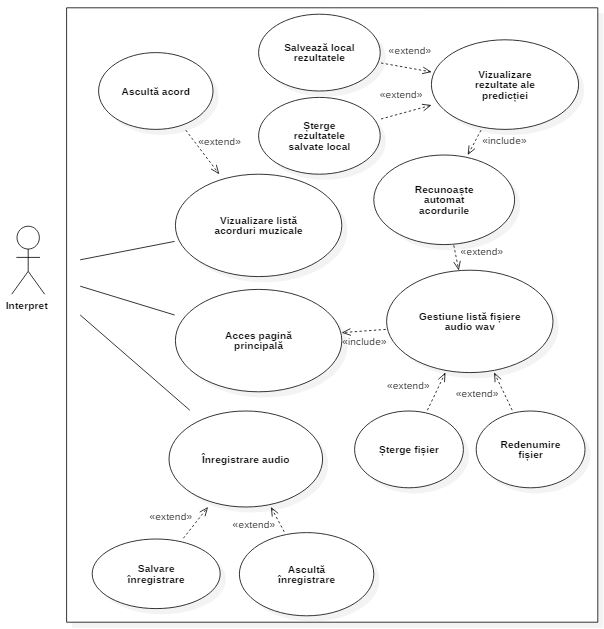
\includegraphics[width=14cm]{..//resources//images//cazuri_de_utilizare_v3.JPG} 
    \caption{Diagrama cazurilor de utilizare, ilustrând actorul ca "Interpret"
și fluxul de evenimente dintre actor și sistem.}
\end{figure}
\newpage

Un alt model important este cel dinamic, care descrie modul în care grupuri 
de obiecte colaborează în cadrul aceluiași eveniment. Specificarea 
modelului se face prin intermediul unei diagrame de interacțiune. 
Există două tipuri de diagrame de interacțiune: diagramele de secvență 
și diagramele de comunicare. Cele două tipuri de diagrame 
sunt echivalente, astfel cunoscându-se o diagramă de secvență, se poate
construi diagrama de comunicare, și reciproc \cite{Ingineria-sistemelor-de-programare}. Pentru exemplificare, 
se va utiliza diagrama de secvență.

Diagramele de secvență au rolul de a reprezenta interacțiuni
între obiecte. Obiectele participante sunt desenate sub formă de dreptunghiuri,
fiind reprezentate pe orizontală, axa timpului fiind pe verticală.
Coloana cea mai din stânga corespunde actorului care declanșează acțiunea.
Acțiunea care este declanșată trebuie să corespundă cu un caz de utilizare 
definit în prima etapă \cite{Ingineria-sistemelor-de-programare}.
Figura 6.2 prezintă diagrama de secvență aferentă cazului de utilizare 
corespunzătoar procesului de recunoaștere automată a unei partituri muzicale 
dintr-o piesă acustică.

\begin{figure}[h!]
    \centering
    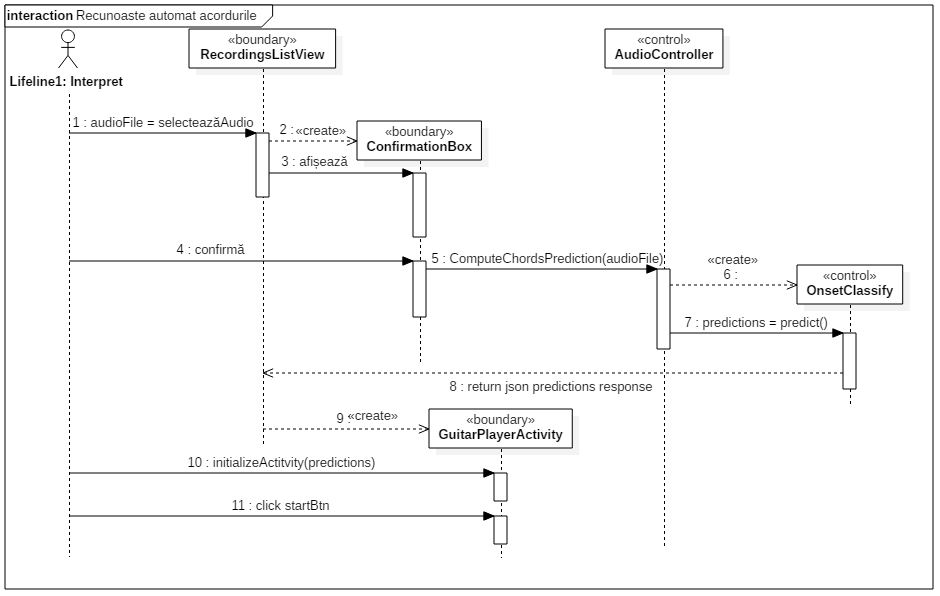
\includegraphics[width=15.8cm, height=10.5cm]{..//resources//images//diagrama_de_secventa2.JPG} 
    \caption{Diagrama de secvență a cazului de utilizare "Recunoaște 
    automat acordurile". }
\end{figure}
\newpage

Ultimul model, modelul obiectual, descrie structura sistemului 
apelând la obiecte, atribute, asocieri și operații \cite{Ingineria-sistemelor-de-programare}. 
Diagrama de clase este implicată în descrirea modelului, fiind compusă dintr-un 
graf, ale cărui noduri reprezintă clasele sistemului construit, 
și ale cărui arce determină relațiile între clase. 
Clasele sunt reprezentate în UML folosind dreptunghiuri cu 3
compartimente (numele clasei, atributele și operațiile), în timp
ce arcele pot fi de mai multe tipuri, în funcție de specificul
legăturii (asociere, agregare, generalizare, compoziție). 

Diagrama de clase aferentă sistemului construit cu scopul automatizării  
procesului de detectare și recunoaștere a acordurilor muzicale este prezentată în Figura 6.3.

Se observă că structura proiectului, pe baza diagramei de clase, nu 
este foarte complexă. Acest aspect este datorat faptului că sistemul 
nu urmează șablonul clasic de MVC, având în vedere noțiunile abordate, și 
etapele necesare de parcurs în modelarea și antrenarea unei rețele neuronale.
Structura este adaptată pe aceste etape, proiectul fiind de 
natură științifică \emph{(Python-Based Data Science Project)}.
Astfel, structura simplă a modelului obiectual este rezultatul aplicării
etapelor (modulelor) care au realizat procesarea datelor audio, extragerea 
trăsăturilor muzicale și constuirea rețelei neuronale convoluționale.

\begin{figure}[h!]
    \centering
    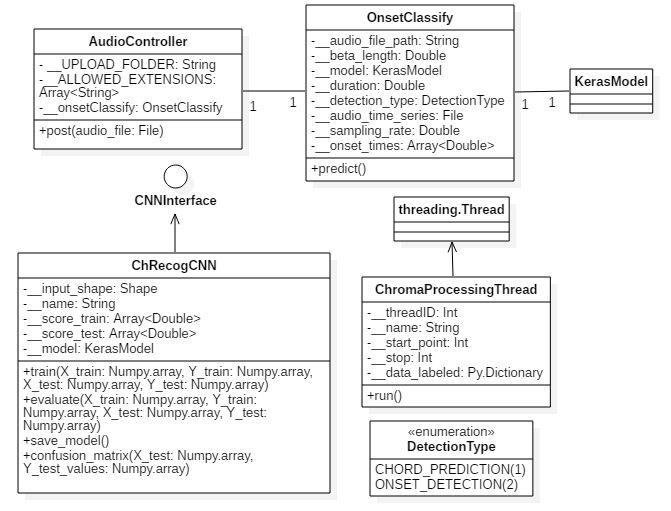
\includegraphics[width=15.8cm]{..//resources//images//class_diagram.JPG} 
    \caption{Diagrama de clase.}
\end{figure}
\newpage

Modulele care compun structura proiectului științific urmează o secvență 
de pași în mod logic, pornind de la module care se aplică exclusiv setului de date, 
continuând cu cele care îmbină datele cu modelul neuronal și terminând cu 
module care sunt destinate doar rețelelor neuronale. Acestea sunt următoarele:
\begin{itemize}
    \setlength\itemsep{0.2em}
    \item Intermediate: modul care se ocupă de procesarea 
    datelor și obținerea unor informații și grupări intermediare;
    \item Processing: la nivelul acestui modul s-a realizat augmentarea datelor 
și s-a testat pentru prima oară detectația tranzițiilor muzicale;
    \item Modelling: în acest pas s-a aplicat transformata Q constantă asupra 
fiecărei înregistrări audio, obținând o listă de chromagrame. Tot aici s-au 
modelat mai multe arhitecturi convoluționale, ajungând treptat la cea mai 
bună soluție;
    \item Model evaluation: modul care utilizează rețeaua antrenată pentru a
furniza predicții și pentru a detecta tranzițiile muzicale, în funcție de 
input-ul dat;
    \item Utils: conține elementele comune proiectului, ca metricile de calcul,
inițializarea jurnalului sau constantele utilizate;
    \item Rest: la nivelul acestui pachet se găsesc endpoint-urile REST API,
disponibile la nivelul controller-ului AudioContoller. Acest modul interacționează
cu modulul de evaluare. 
\end{itemize}

Cunoscând rolurile îndeplinite de fiecare modul (pachet) în parte, se 
poate construi o diagramă care să reprezinte dependențele existente 
între aceste module, dar și componența lor, prin precizarea conținutului
(fișiere python ce pot fi rulate independent, clase sau alte obiecte).
Figura 6.4 modelează întreg ansamblul enunțat. 

\begin{figure}[h!]
    \centering
    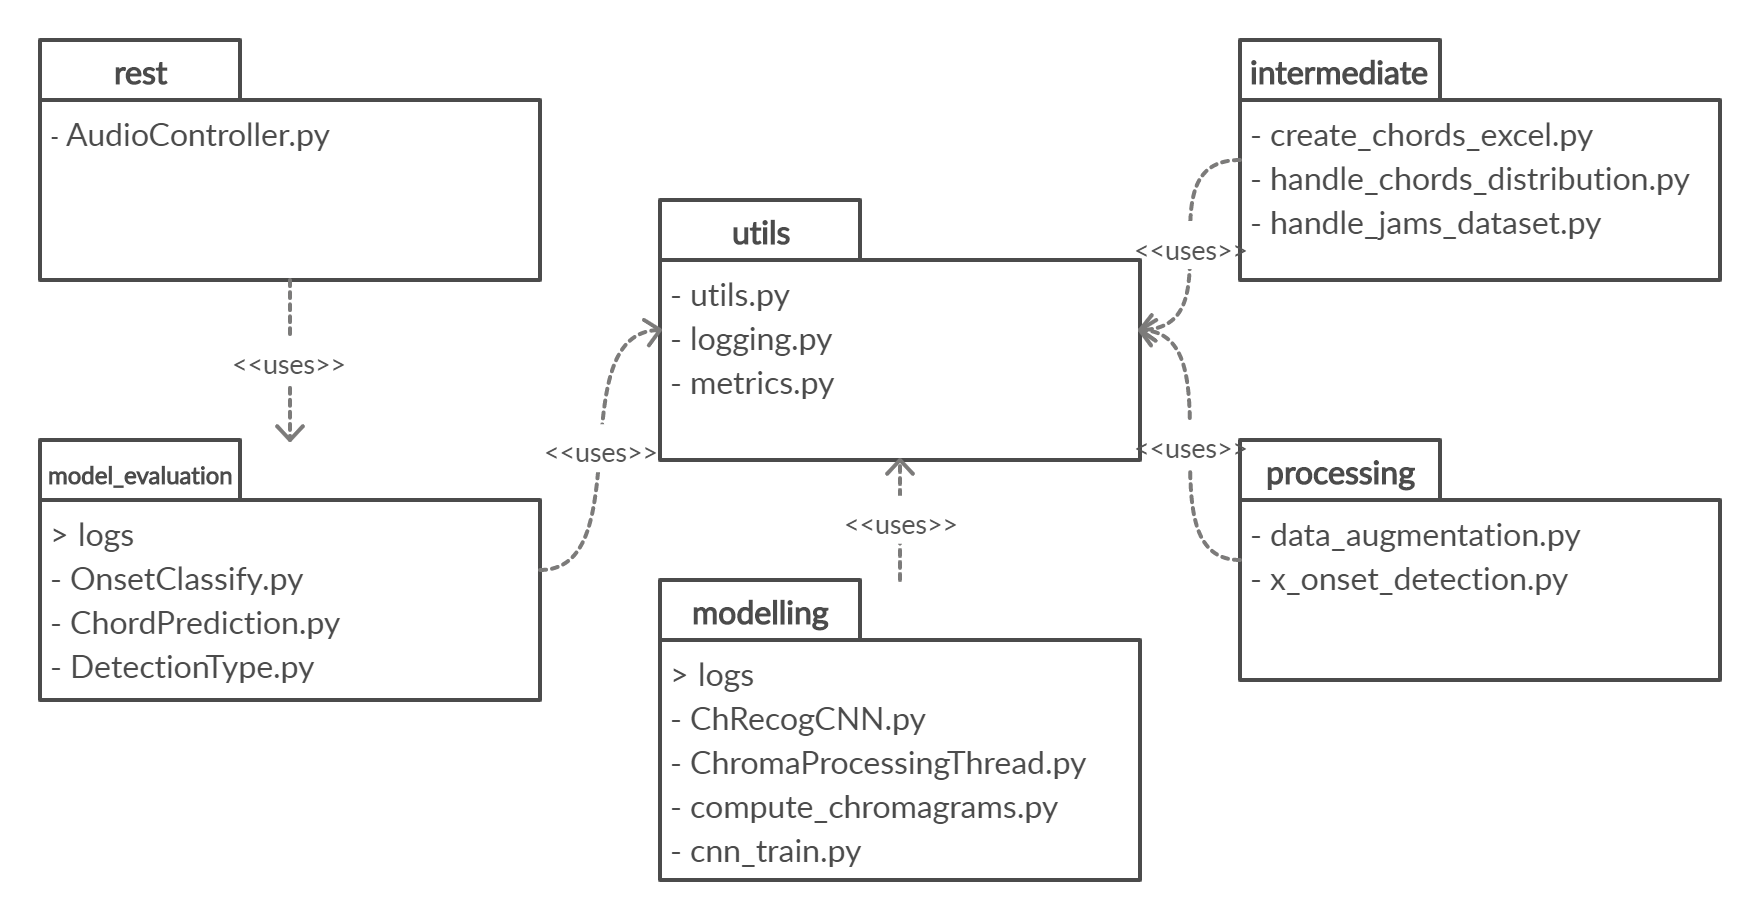
\includegraphics[width=15.8cm]{..//resources//images//packages_diagram2.png} 
    \caption{Împărțirea sistemului pe module, împreună cu 
    dependențele existente.}
\end{figure}
\newpage

\iffalse
\subsection{Evaluarea modelului}

The F1-score can be interpreted as
a weighted average of recall and precision, and an ideal F1-score
would be 1.0, while the worst would be 0.0 [11]. In particular, if
we let TP denote the number of true positives, FN denote the
number of false negatives, and FP denote the number of false
positives.

Metrici

\begin{equation*}
    Recall (R) = \frac{TP}{TP+FN} 
\end{equation*}

\begin{equation*}
    Precision (P) = \frac{TP}{TP+FP} 
\end{equation*}

\begin{equation*}
    F1-score = \frac{2 \cdot R \cdot P}{R + P} 
\end{equation*}
\fi

\section{Aplicația mobile}
În această secțiune se vor prezenta funcționalitățile aplicației mobile 
și modul de realizare a acestora, din perspectiva cazurilor de utilizare 
care determină modelul funcțional al sistemului.
\subsection{Arhitectura aplicației mobile}
Pentru construirea aplicației mobile am ales modelul de proiectare 
MVVM (Model-View-ViewModel). Este unul din cele mai bune modele de design 
care pot fi utilizate pentru a dezvolta o aplicație Android. Acesta 
este construit din: Model, View și ViewModel \cite{WEBSITE:android-mvvm}.

Pachetul Model conține toate clasele care modelează datele prelucrate 
în aplicație, API-uri dar și obiectele de tip Repository. Astfel, aplicația 
folosește un obiect WebRepository care implementează funcționalitățile 
cerute de end-pointurile din WebAPI. 

Acesta interacționează cu pachetul 
de networking, pentru a realiza cererile dorite, cu ajutorul 
clientului REST pentru Java și Android, și anume Retrofit. 
Retrofit face foarte ușor procesul de obținere sau încărcare a unui JSON 
printr-un serviciu web bazat pe REST. Este necesară doar specificarea unui 
convertor pentru serializarea datelor. Retrofit folosește biblioteca OkHttp 
pentru solicitările HTTP.

De asemenea, acest pachet interacționează și cu baza de date locală a telefonului. Entitățile 
sistemului pot fi salvate, la dorința utilizatorului, într-o bază de date 
relațională, prin librăria Room. Room este o librărie de tip 
ORM \emph{(Object Relational Mapping)} care transformă automat tabelele SQLite
în obiecte Java/Kotlin. Permite validarea SQL în timpul compilării 
și returnează obiecte observabile de tip RxJava, LiveData sau 
Flowable \cite{WEBSITE:android-room}.

În cadrul pachetului View se regăsesc structura și aspectele UI cu care 
utilizatorul poate interacționa. Elementele de view sunt construite prin 
fragmente și activități. 

Activitatea este o componentă crucială a unei aplicații Android. Spre 
deosebire de alte paradigme de programare în care aplicațiile sunt 
lansate prin intermediul unei metode principale \emph{main()}, sistemul 
Android inițializează codul într-o instanță de tip activitate, invocând 
metode de apelare specifice care corespund unor etape din ciclul de viață
a unei activități. Aplicația conține două activități: MainActivity - 
activitatea principală, care se lansează la pornirea aplicației, și 
GuitarMusicPlayerActivity - activitate care se ocupă de procesarea 
rezultatelor obținute prin trimiterea unei înregistrări audio către 
sistemul de BE, ce se ocupă cu extragerea trăsăturilor muzicale și 
furnizarea predicțiilor aferente intervalelor muzicale \cite{WEBSITE:android-activity}.

Fragmentele sunt porțiuni de interfață din cadrul unei activități.
Poate fi considerat o secțiune modulară a unei activități, care are 
propriul ciclu de viață, fiind gestionat individual de o activitate.
Aplicația conține 3 fragmente: HomeFragment - pentru gestiunea 
înregistrărilor audio salvate local, RecordingFragment - conține 
un layout care permite înregistrarea unei partituri muzicale, 
folosind microfonul telefonului, și ChordsFragment - fragment 
ce conține un grid layout cu reprezentările grafice a tuturor
acordurilor recunoscute de către sistem.

Pachetul ViewModel este responsabil de traducerea datelor 
din Model într-un format corespunzător pentru View. ViewModel
și View sunt asociate prin mecanismul de legare a datelor \emph{(data 
binding)}, astfel încât orice modificare petrecută la nivel de 
ViewModel, se poate reflecta automat la nivel de View. Prin urmare, 
există câte un ViewModel pentru fiecare activitate/fragment 
existent în aplicație (în afară de MainActivity), prin intermediul cărora
se gestionează elementele vizuale din cadrul fragmentelor și a 
activităților care compun interfața aplicației. 

Relațiile de dependență între pachetele modelului 
sunt reprezentate în Figura 6.5.

\begin{figure}[h!]
    \centering
    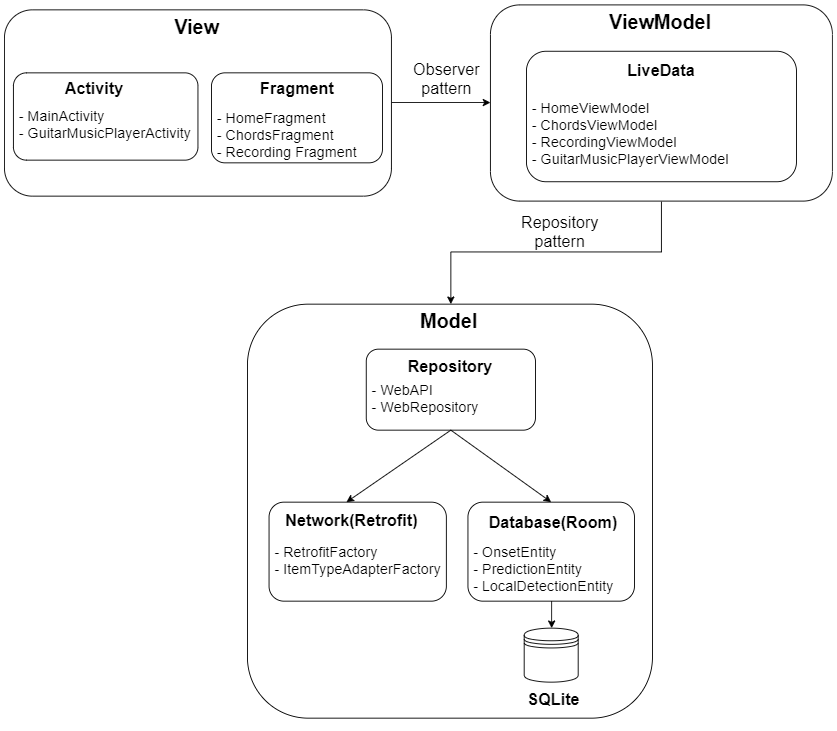
\includegraphics[width=14cm]{..//resources//images//mvvm_mobile2.png} 
    \caption{Prezentarea modelului de proiectare MVVM al aplicației.}
\end{figure}

\newpage
\subsection{Funcționalități}
Aplicația mobile este construită în jurul ansamblului care se 
ocupă de recunoașterea automată a partiturilor muzicale acustice,
având scopul de a pune în evidență funcționarea sistemului 
de recunoaștere. De asemenea, punerea în evidență a sistemului 
trebuie să fie în armonie cu dorințele utilizatorului, astfel încât 
să rezulte un ansamblu complex, care să satisfacă nevoile acestuia, 
în primul rând prin furnizarea unor rezultate corecte, dar și prin
interpretarea acestora într-o manieră simplă și sugestivă, printr-o 
reprezentare grafică din domeniul muzical.

Funcționalitățile aplicației mobile determină modelul 
funcțional al sistemului, fiecare caz de utilizare 
fiind implementat la nivelul unei activități sau a unui
fragment al aplicației. Astfel, activitatea principală 
(MainActivity) este cea care se deschide la pornirea aplicației,
si cuprinde 3 fragmente: HomeFragment, RecordingFragment și 
ChordsFragment. 

Fragmentul principal, care este lansat inițial 
(cazul de utilizare "Acces pagină principală"), este
HomeFragment. Acest fragment are în componență o listă formată 
din înregistrările muzicale aflate în directorul aplicației 
mobile (cazul de utilizare "Gestiune listă fișiere audio wav").
Fiecare element din listă este compus din numele fișierului 
audio, durata acestuia (minute:secunde), un buton lateral 
format dintr-o imagine cu 3 linii, prin apăsarea căruia se 
deschide un submeniu, care oferă posibilitatea de ștergere 
(cazul de utilizare "Ștergere fișier") sau redenumire 
(cazul de utilizare "Redenumire fișier") a fișierului wav.
Opțional, elementul poate conține o imagine cu o bifă, ce sugerează 
faptul că, pentru acel element, informațiile în ceea 
ce privește recunoașterea automată au fost stocate 
în baza de date locală a telefonului.

Având aceste informații setate în mod corespunzător pentru 
fiecare element din listă, se poate realiza cu succes 
recunoașterea automată a acordurilor muzicale. Pentru 
a începe acest proces, este nevoie ca utilizatorul 
să țină apăsat unul din elemente pentru două secunde. 
Acest gest va determina trimiterea fișierului audio ales
către sistemul de recunoaștere, care va realiza operațiile 
necesare, și va întoarce predicțiile determinte sub 
forma unui răspuns JSON (cazul de utilizare "Recunoaște 
automat acordurile"). Acest gest determină și 
schimbarea layout-ului. Astfel, peste fragmentul 
creat, se va instanția și afișa activitatea responsabilă 
de gestiunea rezultatelor sistemului de recunoaștere.
Aceată activitate este GuitarMusicPlayerActivity.

Noua activitate instanțiată este responsabilă de
afișarea rezultatelor obținute într-un mod cât 
mai sugestiv. Astfel, activitatea va gestiona un 
obiect de tip MediaPlayer, care conține fișierul 
audio de tip wav. Acesta va permite redarea 
conținutului audio. În momentul în 
care se pornește conținutul audio, în paralel,
dar în același timp în mod sincronizat, se 
vor afișa, cu ajutorul reprezentării prin tabulatură, 
top 3 acorduri muzicale prezise de către sistemul 
de recunoaștere automată (cazul de utilizare 
"Vizualizare rezultate ale predicției"). 
Acordurile afișate sunt 
cele care se potrivesc intervalului muzical din momentul 
redării (momentul $t_i$), ceea ce determină o schimbare permanentă
a acordurilor afișate, pentru fiecare interval muzical detectat 
de către sistem (momentele $t_{i+1}, t_{i+2}\dots$).  

Fiecare acord muzical reprezentat grafic va fi însoțit 
de o valoare numerică procentuală, ce reprezintă 
probabilitatea asociată predicției de către sistem. 
Astfel, pentru a avea o vedere mai de ansamblu asupra rezultatelor 
pentru fiecare interval muzical, s-a ales afișarea și 
interpretarea primelor 3 predicții.

Tot în această activitate se găsește și opțiunea de a salva/șterge
în/din baza de date locală, rezultatele obținute pentru fișierul audio curent.
Dacă se alege salvarea rezultatelor pentru acest fișier audio, în viitor,
când se va dori din nou o vizualizare a predicțiilor corespunzătoare, 
acestea vor fi luate și afișate din baza de date locală, fiind disponibile 
mult mai rapid, întrucât procesul complex de recunoaștere și furnizare 
a răspunsului din partea sistemului de recunoaștere nu mai are loc. 
Sumarizarea funcționalităților enunțate este redată prin Figura 6.6, 
care prezintă cele două layere descrise, HomeFragment și GuitarMusicPlayerActivity.

\begin{figure}[h!]
    \centering
    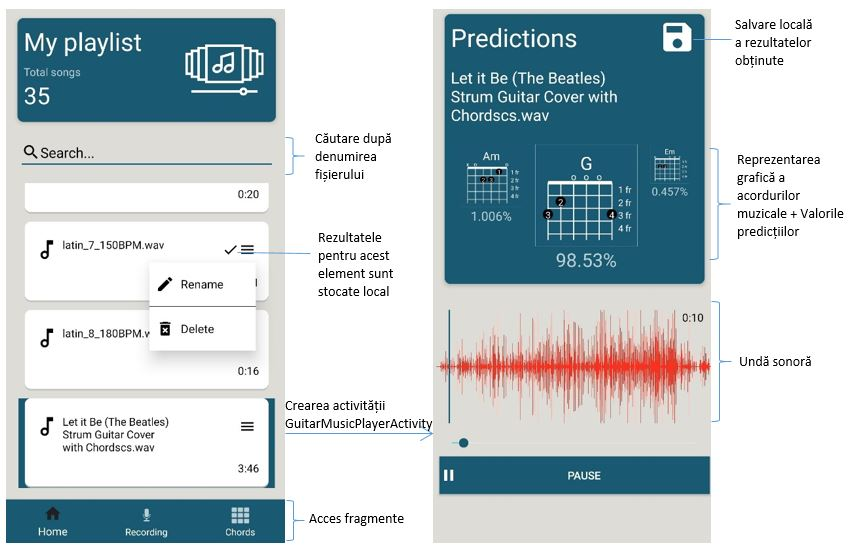
\includegraphics[width=15.8cm]{..//resources//images//mobile_1_v2.jpg} 
    \caption{Imaginea din stânga prezintă elementele fragmentului HomeFragment. 
    Prin ținerea apăsată a unuia din elemente, se instanțează și apoi se 
    afișează activitatea GuitarMusicPlayerActivity (imaginea din dreapta), responsabilă 
    de procesarea și afișarea rezultatelor furnizate de sistemul de recunoaștere 
    automată. }
\end{figure}

Cele două elemente de View prezentate sunt cele mai importante, 
fiind în legătură strânsă cu sistemul de recunoaștere automată a 
partiturilor muzicale. Pe langă ele, mai există în aplicație 
două fragmente auxiliare, anume RecordingFragment și ChordsFragment.

Fragmentul de recording permite utilizatorului să folosească 
microfonul telefonului (sau un microfon extern atașat) pentru 
a înregistra o partitură muzicală (cazul de 
utilizare "Înregistrare audio"). Odată ce acesta 
finalizează înregistrarea, poate să salveze conținutul sub 
forma unui fișier wav, care va fi stocat în directorul 
aplicației, sau să șteargă conținutul și să reîncerce 
realizarea unei înregistrări (cazurile de utilizare "Salvare înregistrare" 
și "Ascultă înregistrarea"). Ulterior, poate folosi 
înregistrea pentru a descoperi acordurile muzicale, prin trimiterea 
acesteia către sistemul de recunoaștere automată.

Ultimul fragment, ChordsFragment, are un 
rol didactic în cadrul aplicației. Fragmentul conține 
o listă cu elemente dispuse sub forma unei grile \emph{(grid layout)},
fiecare element reprezentând unul din cele 24 de acorduri 
recunoscute de către sistem. Astfel, fiecare element din listă prezintă 
numele acordului muzical, împreună cu reprezentarea lui 
grafică (desenul), fiind folosită notația prin tabulatură
(cazul de utilizare "Vizualizare listă acorduri 
muzicale"). Prin selectarea unui element 
din listă, se afișează o fereastră 
de tip popup, care prezintă acordul, și un buton 
de start. Prin apăsarea butonului, dispozitivul mobil 
redă un sunet de aproximativ 2 secunde, ce reprezintă acordul 
muzical selectat, interpretat la o chitară acustică (cazul 
de utilizare "Ascultă acord").
Figura 6.7 ilustrează cele două fragmente descrise mai sus.
\begin{figure}[h!]
    \centering
    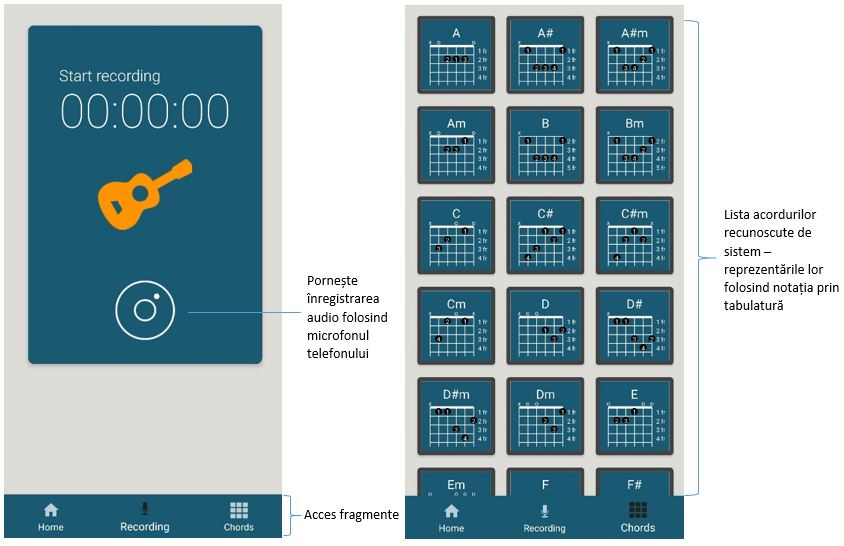
\includegraphics[width=15.8cm]{..//resources//images//mobile_2_v2.jpg} 
    \caption{Imaginea din stânga reprezintă fragmentul RecordingFragment, 
    responsabil de înregistrarea audio, în timp ce imaginea din dreapta 
    prezintă lista acordurilor muzicale recunoscute de către sistem 
    (folosind notația prin tabulatură).}
\end{figure}

\iffalse
\newpage
\subsection{Proiectarea interfeței grafice}
Atât interfața grafică, cât și aspectul aplicației mobile,
au fost proiectate folosind fișiere XML. Folosind vocabularul 
XML oferit de Android, se pot proiecta rapid diverse layout-uri 
pentru interfața grafică, împreună cu elementele corespunzătoare,
în același mod în care se creează pagini Web în HTML - cu o serie 
de elemente imbricate.

Fiecare fișier de layout trebuie să conțină exact un element 
rădăcină, care trebuie să fie un obiect View sau ViewGroup.
După ce se definește obiectul rădăcină, se pot adăuga obiecte 
sau elemente suplimentare ca elemente "copii", în 
raport cu rădăcina, pentru a construi treptat o 
ierarhie de vizualizare care să definească layout-ul \cite{WEBSITE:android-layouts}.
În ceea ce privește rădăcina, cele mai frecvente alegeri 
sunt layout-urile următoare: LinearLayout, ConstraintLayout 
sau RelativeLayout. De asemenea, la nivel de elemente 
componente, se utilizează frecvent elemente ca: 
TextView, Button, ImageView sau ListView \cite{WEBSITE:android-layouts}. 

Fiecare obiect View acceptă propria varietate de atribute.
Unele atribute sunt specifice unui obiect (de exemplu TextView, care 
acceptă atributul textSize), dar pot exista și atribute 
comune (cum ar fi atributul id). De asemenea, există atribute 
considerate "parametrii de layout", acestea având rolul de a descrie 
anumite orientări de layout ale acelui obiect, valori care se bazează 
și pe parametrii setați de obiectul părinte.

În ceea ce privește fișierele xml care definesc 
layout-ul aplicației (4 fișiere, 3 pentru fragmente și 
unul pentru o activitate), acestea au folosit în 
ierarhizare mai multe tipuri de componente, 
pentru a da un aspect plăcut și modern aplicației.
Se consideră ca exemplu, cel mai complex fragment, și 
anume HomeFragment. Acesta este format dintr-un 
LinearLayout (ca rădăcină), având în componență un view de tip 
CardView (compus dintr-o ierarhie de LinearLayout-uri, TextView-uri 
și un ImageView), un EditText (pentru realizarea filtrării), și un 
layout de tip include, care determină integrarea unei liste din 
exterior (dintr-un alt fișier xml). Următoarea secțiune de cod prezintă 
o sumarizare a componentelor enunțate, și a modului de compunere a acestui 
layout.

\lstset{language=XML, numbers=none, frame=single, showstringspaces=false}
\begin{lstlisting}
    <LinearLayout
        android:layout_width="match_parent"
        android:layout_height="match_parent"
        android:background="#DDDCD7"
        android:orientation="vertical">
        <androidx.cardview.widget.CardView
            android:layout_width="match_parent"
            android:layout_height="150dp"
            ...
            <LinearLayout ...
                <LinearLayout ...
                    <TextView ...
                        android:text="My playlist"
                        android:textSize="32dp" />
                    ...
                </LinearLayout>
                <ImageView ... />
            </LinearLayout>
    </androidx.cardview.widget.CardView>
    <EditText ...
        android:hint="Search..." 
        .../>
    <include
        layout="@layout/listview"
        ... />
    </LinearLayout>
\end{lstlisting}

Acest stil de realizarea a unui 
layout este similar și pentru construcția fragmentelor 
rămase. Componentele utilizate sunt aceleași, 
diferă doar ordinea lor, dar și atributele utilizate.
Dacă în ceea ce privește fragmentele, domină 
layout-ul de tip LinearLayout (atât ca rădăcină, cât 
și ca element în structura ierarhică), situația este 
puțin diferită pentru activitate. Activitatea 
GuitarMusicPlayerActivity este formată dintr-un 
ConstraintLayout (ca rădăcină) ce are 
în componență elemente de tip LinearLayout, TextView, 
ImageView și CardView. Spre deosebire de
LinearLayout, care ierarhizează componentele 
în mod liniar, după orientarea aleasă 
(orizontal sau vertical), pentru fiecare 
element din cadrul unui ConstraintLayout trebuie 
precizate constrângerii în relație cu 
componentele vecine (atribute de tipul 
layout{\_}constraint) \cite{WEBSITE:android-layouts}. Modul de definire a unui 
layer de tip Constraint se poate observa prin
secțiunea de cod ce urmează:
\lstset{language=XML, numbers=none, frame=single, showstringspaces=false}
\begin{lstlisting}
    <androidx.constraintlayout.widget.ConstraintLayout
        android:layout_width="match_parent"
        android:layout_height="match_parent"
        android:background="#DDDCD7"
        tools:context=".ui.music_player.GuitarMusicPlayerActivity">

        <androidx.cardview.widget.CardView
            android:id="@+id/cardView2"
            android:layout_width="match_parent"
            android:layout_height="360dp"
            .../>
        <LinearLayout
            android:layout_width="match_parent"
            android:layout_height="wrap_content"
            android:orientation="vertical">
            ...
        </LinearLayout>
    </androidx.constraintlayout.widget.ConstraintLayout>
\end{lstlisting}
\fi

\chapter{Abordări existente pentru recunoașterea automată a partiturilor muzicale}
Ultimii 20 de ani au adus numeroase abordări în ceea ce privește recunoașterea automată
a partiturilor muzicale. De la recunoașterea individuală a instrumentelor muzicale, până
la recunoașterea completă a notelor și diferențierea instrumentelor dintr-o piesă 
completă, s-au încercat diferite metode, în funcție de cantitatea de date disponibilă
până în acel moment, dar și de evoluția tehnologiei.

Una dintre primele lucrări care a stat la baza abordărilor ulterioare pentru o perioadă
de timp este lucrarea propusă de către Sheh și Ellis \cite{Chord-Segmentation-and-Recognition-using-EM-Trained-HMM}.
Metoda are la bază învățare statistică utilizând modele Markov cu stări ascunse. 
Antrenarea modelului s-a realizat folosind algoritmul EM, tratând etichetele pentru
acorduri ca valori ascunse pentru construcția EM. Tot pentru antrenarea modelului
au folosit doar secvența de acorduri (\emph{without chord boudaries} - neclasificate, în
raport cu intervalele de timp în care se găsește un anumit acord) ca
input pentru modelul Markov, aplicând astfel algoritmul Baum-Welch pentru a estima parametrii
modelului. Algoritmul garanta că estimările se vor îmbunătăți de la o etapă la alta, ajungând
într-un optim local, în ceea ce privește setul de parametrii. 
După determinarea parametrilor,
asupra modelului se aplică algoritmul lui Viterbi, pentru a afla cea mai optimă cale(cea
mai probabilă secvență de acorduri pentru un semnal audio de intrare).

Rezultatele obținute au fost: 76\% pentru precizia segmentării acordurilor din
piese și 22\% pentru precizia în recunoașterea acordurilor. Performanța scăzută pentru
recunoaștere se datorează faptului că datele de antrenare au fost neclasificate, dar și 
faptului că acestea au fost insuficiente (20 de melodii pentru 147 de acorduri).

Plecând de la această abordare, aproximativ 3 ani mai târziu, Lee și Slaney au enunțat
o metodă îmbunătățită \cite{Automatic-Chord-Recognition-from-Audio-Using-an-HMM-with-Supervised-Learning}, 
având un set de date adnotat și mai numeros, compus din 140 de melodii,
obținând o precizie de 93.35\% în recunoașterea acordurilor, din cadrul melodiilor
testate.

Începând cu anul 2009, odată cu apariția unui 
set de date compus din piese de pe diverse albumuri aparținând trupelor Beatles, Zweieck 
sau Queen, complet adnotate cu acorduri, strategia în rezolvarea acestei probleme s-a schimbat,
și foarte multe lucrări au utilizat acest set de date, aplicând diverse metode și comparând rezultate.

O primă lucrare care a abordat mai multe strategii de clasificare, dar și de procesare sonoră,
a fost lucrarea de masterat a lui Alessandro Bonvini, din anul universitar 2012-2013, \cite{Bonvini-Recognition}.
În ceea ce privește algoritmii de învățare automată, a abordat problema utilizând 
3 metode, și anume: regresie logistică (LgR), construirea unui ANN, având un singur strat ascuns 
\emph{(Single Hidden Multilayer Perceptron, MPL)} și construirea unei rețele de convingeri profunde (DBN).

Bonvini a prezentat rezultatele comparativ, aplicând mai multe strategii de normalizare a datelor,
testând la fiecare schimbare toți algoritmii. Se vor prezenta rezultatele obținute 
prin aplicarea strategiei de normalizare $L-\infty$. În ceea ce privește metricile de evaluare 
a performanței, a introdus două valori specifice numite Weighted Average Overlap Ratio(WAOR),  
indicând durata de timp în care segmentele clasificate în mod corect rămân suprapuse 
celor din realitate, și Segmentation Quality (SQ), sugerând calitatea segmentării (Tabelul 7.1).

\iffalse
Rezultatele obținute au fost: 
\begin{itemize}
    \item LgR: WAOR: 66.9\%, SQ:  74.1\%;
    \item MPL: WAOR: 69.6\%, SQ:  74.9\%;
    \item DBN: WAOR: 71.9\%, SQ:  76.0 \%.
\end{itemize}
\fi

\begin{table}[h!]
    \begin{center}
        \begin{tabular}{ | c | c | c | }
            \hline 
                Algoritm & Weighted Average Overlap Ratio & Segmentation Quality\\
                \hline \hline 
                LgR & 66.9\% & 74.1\% \\
                \hline
                MPL & 69.6\% & 74.9\% \\
                \hline
                DBN & 71.9\% & 76.0\% \\
            \hline
        \end{tabular}
        \caption{Rezultatele obținute de Bonvini în lucrarea de masterat.}
    \end{center}
\end{table}

Tot în preajma anului 2012, în cadrul Conferinței Internaționale de Machine Learning din Florida, SUA,
s-a prezentat o lucrare care avea să schimbe încă odată direcția de a aborda problema 
recunoașterii automate a acordurilor, prezentând rețelele neuronale convoluționale 
ca o soluție cu eficiență ridicată, prin comparație cu abordările anterioare, în special
prin referire la modelele Markov. 

Lucrarea propusă de către Humphrey și Bello, \cite{Rethinking-Automatic-Chord-Recognition-with-CNN}, 
descrie două arhitecturi convoluționale, prezentând construcția strat cu strat și 
strategia antrenării. O precizare importantă este aceea că, în privința procesării audio și 
a extragerii de trăsături nu a existat o schimbare, metoda aleasă fiind transformarea Q constantă. 
Setul de date utilizat conține 475 de înregistrări audio, 
însumând aproximativ 50000 de acorduri diferite.

Antrenând și testând cele două rețele convoluționale, s-a obținut 77.4\%, respectiv 
76.8\% acuratețe la testare, demonstrând că această abordare performează într-un mod competitiv 
cu alte abordări considerate consacrate până în acel moment.

Începând din acel moment, majoritatea lucrărilor au propus metode pe baza 
rețelelor neuronale convoluționale. Cea mai concludentă lucrare analizată, prin raportare 
la soluția propusă, este cea prezentată de Zhou și Lerch, \cite{Chord-detection-using-Deep-Learning},
de la centrul pentru tehnologia muzicii, din cadrul institutului de tehnologie din Georgia, SUA.
Lucrarea prezintă construcția a două rețele profunde cu 6 straturi, în două arhitecturii diferite:
o arhitectură clasică, cu același număr de neuroni (1024) în fiecare strat, și o arhitectură de tip 
\emph{bottleneck (cu număr scăzut de neuroni în mijlocul rețelei, și în vecinătatea mijlocului)}. 
Setul de date constă în 317 piese adunate din discografiile unor trupe celebre, fiecare piesă
fiind divizată în peste 1000 de cadre, pentru recunoașterea individuală a acodurilor. 
Algoritmul propus este capabil să recunoască acordurile majore și minore pentru fiecare 
notă de tip rădăcină, rezultând un dicționar de etichete pentru acorduri de dimensiunea 24+1, având
24 de acorduri cu etichete corespunzătoare cunoscute, și o etichetă pentru orice alt acord care 
nu este recunoscut.

Rezultatele obținute sunt prezentate pe ambele arhitecturi, aplicând diferite metode 
de pre-procesare a datelor. Cele mai bune rezultate au fost obținute folosind strategia 
\emph{spliced filters}. Metrica de evaluare a perfomanței este durata totală a segmentelor cu predicție corectă. 
Astfel, rezultatele sunt prezentate în Tabelul 7.2.
\iffalse
\begin{itemize}
    \item Arhitectura comună: 98.5\% la antrenare și 87.6\% la testare;
    \item Arhitectura bottleneck: 93.6\% la antrenare și 91.9\% la testare.
\end{itemize}
\fi

\begin{table}[h!]
    \begin{center}
        \begin{tabular}{ | c | c | c | }
            \hline 
                Etapă &  Arhitectura comună & Arhitectura bottleneck\\
                \hline \hline 
                Antrenare & 98.5\% & 93.6\% \\
                \hline
                Testare & 87.6\% & 91.9\% \\
            \hline
        \end{tabular}
        \caption{Rezultatele obținute de Zhou și Lerch, prin compararea celor două arhitecturi.}
    \end{center}
\end{table}

Se observă o îmbunătățire semnificativă a rezultatelor, construindu-se rețele 
convoluționale tot mai eficiente, creșterea fiind direct proporțională cu
creșterea datelor etichetate corect și în detaliu. 

Evoluția studiului
în domeniu continuă până în preajma perioadei actuale, fiind prezentată o lucrare 
foarte importantă acum aproximativ un an de către 
Nadar, Abeßer și Grollmisch, \cite{Towards-CNN-based-Acoustic-Modeling-of-Seventh-Chords-for-ACR},
în cadrul unei Conferințe de procesare sonoră, de la Malaga. 
Lucrarea urmărește extinderea dicționarului de etichete de la 24 la 84 de acorduri, extinzând
aria claselor de acorduri care pot fi recunoscute. Dacă până acum se recunoșteau doar 
acordurile majore și minore ale notelor rădăcină, în această lucrare se dorește recunoașterea 
altor clase, printre care septacorduri sau acorduri diminuate.
Setul de date este complex, fiind compus atât din clasicele piese din cadrul discografiilor unor 
trupe celebre, cât și dintr-un set de date special pentru chitară, creat de Institutul de semantică
muzicală Fraunhofer, din cadrul Universității Tehnice Ilmenau, Germania. 

Modelul convoluțional prezentat este alcătuit din mai multe straturi convoluționale, intercalate de
straturi de agregare de tip max pooling, rețeaua având un total de 12 straturi. Rețeaua a fost 
construită pentru a aborda două strategii, una care propune recunoașterea pe baza dicționarului 
extins, dar care nu folosește întreg setul de date (S-84), 
și una care folosește dicționarul clasic, cu 24 de acorduri (S-24). 

Metrica folosită este \emph{f-score}. Astfel, cele mai bune rezultate obținute sunt: 76\% pentru stategia 
S-84, folosind doar setul de date al Institutului Fraunhofer, și 91\% prin strategia S-24, folosind întreg setul de date.
\iffalse
\begin{itemize}
    \item S-84: 76\%, folosind doar setul de date al institutului Fraunhofer;
    \item S-24: 91\%, folosind întreg setul de date.
\end{itemize}
\fi

\iffalse
\begin{table}[h!]
    \begin{center}
        \begin{tabular}{ | c | c | }
            \hline 
                Strategie & Scorul F \\
                \hline \hline 
                S-84, dicționar extins & 76\% \\
                \hline
                S-24, dicționar clasic,  & 91\% \\
            \hline
        \end{tabular}
        \caption{Rezultate...}
    \end{center}
\end{table}
\fi

\iffalse
\begin{figure}[h!]
    \centering
    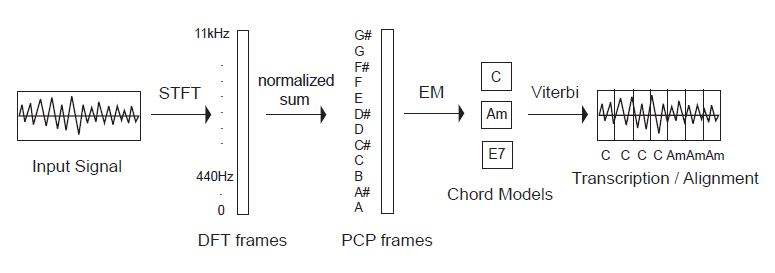
\includegraphics[width=14cm]{..//resources//images//hmm_model.JPG} 
    \caption{}
\end{figure}
\fi

\newpage
\chapter{Concluzii}
\section{Rezumat}
\iffalse
În acestă lucrare am prezentat cele mai adecvate și eficiente metode 
de învățare automată pentru recunoașterea și clasificarea acordurilor 
muzicale acustice. S-au abordat mai multe strategii, de la modele 
probabilistice, până la rețele convoluționale moderne, tratând fiecare 
subiect în parte, în primă fază la nivel teoretic, cu diverse definiții 
sau anumiți algoritmi specifici, prezentând în faza a doua rezultatele celor
mai apreciate lucrări ștințiifice care au abordat aceeași problemă, folosind
unul din metodele enunțate.

Pe baza cercertărilor conexe, am propus o soluție care utilizează
o rețea convoluțională, prezentând arhitectura, setul
de date folosit și rezultatele obținute la antrenare și la testare,
în ultima secțiune a lucrării. Am demostrat astfel eficiența 
și versatilitatea acestui 
model neuronal, care poate fi aplicat cu succes și 
în acest domeniu atât de răspândit.
\fi

În această lucrare s-au prezentat abordări pentru 
problema recunoașterii automate a partiturilor muzicale.
S-a observat că rezolvarea problemei este dependentă 
de parcurgerea a două etape principale. 
Prima etapă se referă la metode de procesare ale 
semnalului sonor, și obținerea unei reprezentări
semnificative.
S-au prezentat aspectele teoretice și practice 
a două metode, trasformata Fourier pe termen scurt și 
transformata Q constantă. În ceea ce privește reprezentarea 
semnalului, s-a ales reprezentarea prin chromagramă, prezentându-se 
tehnicile de compunere.

Etapa a doua este reprezentată de introducerea algoritmilor 
de învățare automată, cu focus pe rețele neuronale profunde. 
Rolul acestora este de a crea un model neuronal bazat pe 
reprezentările înregistrărilor audio, model care 
va fi folosit în clasificarea acordurilor detectate.

Aceste două etape au fost aplicate asupra unui set 
de date format din înregistrări audio de tip wav (fișiere audio 
originale și augmentate). Astfel, pentru procesarea sunetului s-a 
utilizat transformata Q constantă, pe baza căreia s-a obținut 
chromagrama fiecărui fișier audio. Cu lista de chromagrame 
(matrici de caracteristici) construită, pentru pasul următor, 
s-a construit, antrenat și evaluat o rețea neuronală convoluțională. 
Prin analiza rezultatelor obținute pentru 
metricile de calcul și prin analiza graficelor, 
s-a observat că acest model furnizează rezultate excelente, fiind 
o alegere foarte bună pentru acest domeniu. Modelul neuronal a fost 
combinat cu un algoritm de detecție a tranzițiilor muzicale, pentru 
a face posibilă recunoașterea partiturilor 
pe intervalele muzicale observate, obținând astfel 
rezultate complete și corecte pentru întreg conținutul 
muzical.

Pe baza sistemului de recunoaștere construit, s-a realizat și o 
aplicație mobile destinată utilizatorilor care îndrăgesc muzica 
acustică la chitară. Aplicația permite gestiunea unui 
playlist de piese acustice, care pot fi trimise, 
la dorința utilizatorului, către sistemul de recunoaștere, 
care va întoarce rezultatele prezise, aplicația având 
rolul de a reprezenta grafic aceste rezultate, utilizând notația prin 
tabulatură. Aplicația mai permite înregistrarea unei piese, folosind 
microfonul telefonului. De asemenea, mai pune la dispoziția utilizatorului 
o listă cu toate reprezentările sub formă de tabulatură recunoscute 
de către sistem, având un scop didactic pentru cei dornici să 
învețe modul de realizare la chitară a acordurilor muzicale.

\section{Îmbunătățiri viitoare}
Calitatea clasificării obținute prin tehnicile de învățare 
automată este strict legată de calitatea 
informațiilor muzicale extrase. Din acest motiv, 
se poate investiga obținerea și 
folosirea unei reprezentări 
mai bune decât chromagrama, prin analiza unor 
metode diferite de procesare a semnalului sonor. Astfel, 
s-ar putea obține o îmbunătățire a trăsăturilor muzicale 
extrase din înregistrările audio acustice.

În ceea ce privește metodele de învățare 
automată utilizate, ar putea fi luată 
în considerare o abordare care să folosească 
un alt algoritm de învățare supervizată. 
S-a observat prin realizarea cercetărilor conexe 
că rețele neuronale de convingeri profunde 
pot furniza rezultate interesante, ceea ce
face ca această arhitectură să merite o analiză 
mai amplă, dar și o implementare pentru 
a îi dovedi calitățile și utilitatea. De asemenea, 
un model neuronal modern care nu este abordat în această 
lucrare este cel al rețelelor neuronale recurente, 
având și ele un rol important în prelucrarea,
modelarea și clasificare imaginilor. 

O altă analiză înspre îmbunătățirea 
sistemului poate fi făcută pentru 
algoritmul de detecție a tranzițiilor muzicale.
Detecția tranzițiilor este o arie separată 
de cea a recunoașterii partiturilor muzicale, 
având numeroase abordări la rândul ei.
Se pot detecta tranzițiile muzicale inclusiv 
prin crearea unei rețele neuronale convoluționale, 
întrucât există seturi de date adnotate corespunzător, 
cu ajutorul cărora se poate realiza un model neuronal 
specializat doar pe obținerea intervalelor muzicale,
intervale care să fie folosite mai departe 
pentru alți algoritmi sau metode. 

Deși rezultatele obținute prin metodele alese 
pentru implementare sunt foarte bune, cu siguranță există 
loc de îmbunătățiri, mai ales dacă se realizează și o 
îmbogățire a setului de date. Recunoașterea automată 
a partiturilor muzicale este o temă cu multiple abordări,
fiecare aducând un element de noutate domeniului.
Este clar că evoluția tehnologiei și a puterii 
de calcul în ceea ce privește învățarea automată 
se va reflecta și asupra acestui domeniu, 
iar în viitor vor exista modele de recunoaștere 
automată tot mai exacte, fiind capabile să acopere 
arii tot mai mari din sfera muzicii 
acustice contemporane, și nu numai.

\newpage
\printbibliography[title=Bibliografie]

\end{document}
